%\documentclass[12pt]{article}
\documentclass[draft,jgrga]{AGUTeX}
%\documentclass[jgrga]{AGUTeX}
\usepackage{amsmath}
\usepackage[dvips]{graphicx}
\usepackage{xcolor}

\authorrunninghead{ZHENG ET AL.}
\titlerunninghead{DNS for Entrainment}

\newcommand{\Eq}[1]{Eq.~\eqref{#1}} \newcommand{\Fig}[1]{Figure~\ref{#1}}
\newcommand{\Sec}[1]{Sec.~\ref{#1}} \newcommand{\Table}[1]{Table~\ref{#1}}

\begin{document}
\title{A New Particle-Resolved Direct Numerical Simulation Model for Studying Turbulent Entrainment-Mixing Processes}
\author{Zheng Gao,\altaffilmark{1}
Yangang Liu,\altaffilmark{2}
Xiaolin Li,\altaffilmark{1}
Chunsong Lu,\altaffilmark{3}}

\altaffiltext{1}{Department of Applied Mathematics and Statistics, Stony Brook University,
Stony Brook, NY 11794--3600, USA}
\altaffiltext{2}{Brookhaven National Laboratory, Upton, NY 11973--5000, USA}
\altaffiltext{3}{Nanjing University of Information Science and Technology, Nanjing, China}

\begin{abstract}
A new particle-resolved three dimensional direct numerical simulation (DNS) model is developed that combines Lagrangian droplet tracking with the Eulerian field representation. Six numerical experiments are performed to investigate the processes of entrainment of clear air and subsequent mixing with cloudy air and their interactions with cloud microphysics. The experiments are designed to represent different combinations of three initial cloudy area configurations (e.g., cloud-top mixing, lateral mixing, and inside clouds) and two turbulence scenarios (decaying and forced turbulence). The results show that even with the same cloud water fraction, the thermodynamic and microphysical properties are highly different with different settings, especially for the decaying cases. The results suggest that the initial shape of cloud filaments should be considered as a significant transient factor in the study of turbulent entrainment and mixing processes and their influences on cloud microphysical properties.   
\end{abstract}

\begin{article}

\section{Introduction}
Reliable knowledge of cloud droplet size distributions and related microphysical properties (e.g., droplet concentration, liquid water content, and relative dispersion) is crucial for many cloud-related areas such as precipitation, weather and climate modeling, and remote sensing. A long-standing problem in cloud physics is that observed droplet size distributions are generally much broader than those predicted by the classical uniform model (e.g., \cite{Howell1949, HudsonYum1997, YumHudson2001, YumHudson2005}. Understanding the issue of so-called spectral broadening has been a fundamental focus of cloud physics over the last decades, and a number of ideas have been proposed, including stochastic condensation theory that considers the growth of droplet populations as a stochastic process and relates the spectral broadening to turbulence-related fluctuations \cite{Zhou1964, Sedunov1974, MacGrawLiu2006, KhvorostyanovCurry1999}; systems theory that applies statistical physics ideas to cloud physics \cite{Liu1995, LiuHallett1997, LiuHallett1998, Liu2002, Yano2016}; turbulence-induced preferential concentration of droplets \cite{Shaw1998}; and turbulent entrainment-mixing processes \cite{Warner1973, Baker1980, Hicks1990, TelfordChai1980, Su1998, Lu2013}. Another outstanding problem is related to the formation of warm rain \cite{McGrawLiu2003,MacGrawLiu2004}. It is observed that precipitation in warm clouds can be initiated within $30$ minutes after cloud formation \cite{RogersYau1996}. However, according to adiabatic condensational growth theory, too much time is required for cloud droplets to grow large enough to initiate the collision-coalescence process and moreover cloud droplet size distribution becomes narrowed as cloud droplets grow, hampering realistically fast growth of cloud droplets to raindrops. 

Despite the progress (see \cite{Devenish2012, GrabowskiWang2013} for recent reviews), details of the processes involved remain poorly understood and elusive. Furthermore, it is commonly accepted that the accuracy and reliability of climate models in projecting the climate change caused by climate forcing depend heavily on cloud feedbacks and thus on representations (parameterizations) of still poorly understood cloud processes, which have the potential to dampen or enhance changes in essential climatic variables such as temperature and precipitation. The situation worsens when interactions with natural and anthropogenic aerosols are included. Indeed, the latest Inter-governmental Panel on Climate Change continues to assigns ``very low confidence'' to aerosol-cloud-precipitation interactions, with even the sign of the resulting climate forcing remaining uncertain. Understanding such complex processes and upscaling them to adequate representation in climate models present additional challenges to the scientific community, which become more acute for extreme precipitation and weather events and as climate models progress to ever-increasing resolutions. In particular, many key processes, including microphysics, turbulent entrainment-mixing between clouds and environmental air, turbulence and their mutual interactions, occur at scales smaller than typical grid sizes of even large eddy simulation (LES) models (e.g., $100$ m) or cloud-resolving models (CRM) (e.g., $1$ km) are either not represented at all or represented in very rudimentary ways, seriously hindering progress of climate and weather modeling and prediction.

Despite their differences, virtually all the ideas tie the outstanding problems to turbulence-related processes that occur on sub-LES scales (e.g. $< 100$ m) such as turbulence-microphysics interactions and turbulent entrainment-mixing processes. There are significant knowledge gaps on such sub-LES scale processes because of the limitations in conventional modeling and observations. Fully addressing these vital knowledge gaps at the fundamental level calls for a particle-resolved direct numerical simulation (DNS) model that not only resolves the smallest turbulent eddies in clouds, but also tracks motion and growth of individual particles as a supplement to measurements. Since the pioneering works in early 2000s \cite{Vaillancourt00, Vaillancourt02}, a few studies have contributed to developing and applying DNS to cloud microphysics. In a series of publications, \cite{And04, And06, And09}, Andrejczuk and his coauthors developed the EULAG model as a DNS to study the cloud-clear air interfacial mixing and effects of mixing processes on cloud microphysics in decaying moist turbulence. They examined the effects of initial turbulence kinetic energy (TKE), cloud fraction, droplet sizes, and the relationship between the mixing mechanisms and the Damk\"{o}hler number. The initial cloud filaments and velocity field were preset to focus on the details of the decaying turbulence. Both bulk microphysics and detailed bin microphysics were used in the model. \cite{Malinowski2008} compared laboratory measurements with the results of \cite{And04, And06}. \cite{LozarMellado2013} added more features such as sedimentation and particle inertial in the bulk formulation. Other researchers explored DNS by treating the droplet field as discrete particles and explicitly tracking these particles. In \cite{Lanotte2009} and \cite{Celani05}, a model combining Eulerian description of the turbulent velocity and supersaturation fields with a Lagrangian population of cloud droplets was used to study the condensation and evaporation of cloud droplets in turbulent flows. A more complicated model was considered in \cite{Vaillancourt00, Vaillancourt02} by including temperature and vapor mixing ratio field. The authors investigated the influence of nonuniformity in the spatial distribution of sizes and positions of cloud droplets on the droplet size distribution. The relationships among preferential concentration, sedimentation and Stokes number were also discussed. The DNS solves the forced incompressible Navier–Stokes equations in 3D by use of the method of \cite{Sullivan1994}. The effect of entrainment-mixing processes on cloud microphysics was not addressed in these studies. Similar to \cite{Vaillancourt02, Lanotte2009, Kumar11, Kumar12} developed a particle resolved DNS to study turbulent entrainment mixing processes. In their work, a slab-like vapor field was adopted to mimic the supersaturated cloudy area and subsaturated environment. The effects of temperature and buoyancy were ignored while an artificial isotropic volume forcing is introduced to maintain the turbulence. In \cite{Kumar14}, the authors extended their previous work to both forced and decaying turbulence, and claimed that the buoyancy due to droplet evaporation played minor role in the mixing process. 

Despite the progress, many questions regarding turbulence-microphysics interactions and turbulent entrainment-mixing processes remain elusive, still posing challenges for fundamentally understanding and representing clouds in coarse-resolution climate model. This work expands on these previous studies with three primary objectives. First, as for the entrainment and mixing study, it is interesting to note that the settings in \cite{Kumar12, And04} are similar, except the initial configuration of the cloudy area. The cloudy area consists of worm-like area determined by the velocity field of the turbulent flow in \cite{And04}, while a slab-like cloud filament is adopted in \cite{Kumar12}. It is expected that differences in the configuration of cloudy area may cause differences in the results. However, no study has been concentrated on such configuration impact. Thus, one of the objectives of this paper is to explore the effects of initial configuration of cloudy area. Second, it has been recently demonstrated that different mixing scenarios can occur and change during one single cloud evolution \cite{And09, Burnet1992, Lehmann09} and therefore it becomes more and more important to have a reasonable and accurate estimation of the mixing scenario for a sub-grid model. \cite{Lu2013} proposed the transition scale number to measure the occurrence probability of homogeneous or inhomogeneous entrainment-mixing process. Both of the cloud observations and numerical simulations imply a positive relationship between the transition scale number and the homogeneous mixing degree. Thus, the second objective is to systematically investigate the potential of unifying the parameterization of mixing types for larger scale models. Last but not least, to the best of our knowledge, all DNS models have been based on pseudo-spectral methods due to its superior accuracy \cite{Rogallo81, Orszag72, Celani05, Kumar12}. However, the standard pseudo-spectral method has some limitations. As claimed in \cite{Kumar12}, the spectral method requires smooth initial conditions to avoid the Gibbs phenomenon, and thus unable to address sharp or zeroth-order discontinuous interfaces that likely exist in real clouds [e.g., \cite{Brenguier1993}. Moreover, the spectral method requires a periodic boundary condition in each direction and thus cannot be applied to flows that require a non-periodic, physical boundary condition. To be flexible enough to deal with various initial profiles with sharp cloud-air interfaces as well as applying different boundary conditions in the future, we develop a new particle-resolved DNS using finite difference method coupled with WENO (Weighted Essentially Non-Oscillatory) scheme \cite{JiangShu1996}, which has the capability of dealing with discontinuity without causing numerical overshoots at sharp interfaces. Thus, the third objective is to develop a new particle-resolved model based on the finite different method for more general application.

The rest of the paper is organized as follows. Section 2 introduces the system of equations and the numerical schemes used to solve these equations. Section 3 describes the design of the numerical experiments, including configurations of different cases studied and initial and boundary conditions for numerical simulations. The results and discussion are provided in Section 4. Concluding remarks are presented in Section 5. 

\section{Description of New Particle-Resolved DNS}\label{particle_dns}

\subsection{Equations of Thermodynamical and Dynamical Fields}

Similar to most previous DNS, our new DNS is based on the incompressible
Boussinesq fluid system \cite{And04}. Briefly, the dynamical field is give by
\begin{subequations}

\begin{equation}
\partial_{t}\mathbf{u}+(\mathbf{u}\cdot\nabla)\mathbf{u}=-\frac{1}{\rho_{0}}\nabla p+\nu\nabla^2 \mathbf{u}+\mathbf{f}_b + \mathbf{f}_e\label{eq:NS1}
\end{equation}


\begin{equation}
\nabla\cdot \mathbf{u}=0\label{eq:NS2}
\end{equation}

\end{subequations}

where $\mathbf{u}$ is the velocity field, $p$ is the pressure field, $\nu = 1.5\times 10^{-5}m^2s^{-1}$ is the kinetic viscosity, $\rho_{0}$ is the density of dry air. Here $\mathbf{f}_b$ is the buoyancy force given by 

\begin{equation}
\mathbf{f}_b= 
-\mathbf{g}[\frac{T-T_{0}}{T_0}+0.608(q_{v}-q_{v0})-q_{c}]
\label{eq:source_term}
\end{equation}

where $\mathbf{g}$ is the gravity, $T$ and $q_{v}$ are temperature
and vapor mixing ratio field respectively with the subscript ``$0$''
denoting the reference value. The force $\mathbf{f}_e$ is introduced as an 
external, ``large" scale forcing to maintain the turbulence, and is determined 
by the low-wavenumber forcing in the Fourier space:

\begin{equation}
\mathbf{f}_e(\mathbf{k},t) = \epsilon_{in}\frac{\mathbf{u}(\mathbf{k},t)}
{\sum_{\mathbf{k}_f\in \kappa}|\mathbf{u}(\mathbf{k}_f,t)|^2}
\delta_{\mathbf{k},\mathbf{k}_f}
\end{equation}

where $\mathbf{u}(\mathbf{k},t)$ is the velocity function in Fourier space, $\mathbf{k}_f$ is chosen from a subset of the wavenumber space $\kappa$ containing a few wavevectors, for example $(2\pi/L_x,2\pi/L_y,4\pi/L_z)$ plus all permutations with respect to components and sign, $\epsilon_{in}$ is the input energy rate \cite{ghosal1995dynamic}. $\delta_{k,k_f}$ is a delta function. Therefore, statistically stationary homogeneous turbulence can be obtained in DNS by forcing the low-wavenumber modes. For decaying turbulence simulations, $\mathbf{f}_e$ is set to zero.

The temperature $T$ and vapor mixing ratio $q_v$ are described by the following equations (\cite{Kumar11}):

\begin{equation}
\partial_{t}T+(\mathbf{u}\cdot\nabla)T=\frac{L_{h}}{c_{p}}C_{d}+\mu_{T}\nabla^{2}T\label{eq:Temp}
\end{equation}
\begin{equation}
\partial_{t}q_{v}+(\mathbf{u}\cdot\nabla)q_{v}=-C_{d}+\mu_{v}\nabla^{2}q_{v}\label{eq:Vapor}
\end{equation}

where $L_{h}$ is the latent heat of water vapor condensation,
$c_{p}$ is the specific heat at constant pressure, $\mu_{T}=\mu_{v}$ are
the molecular diffusivity for temperature and water vapor, respectively
and assumes to be equal to $2.16\times 10^{-5}m^2s^{-1}$. The condensation rate $C_{d}$ denotes the rate of exchange between liquid and vapor, and is described by:

\begin{subequations}

\begin{equation}
C_{d}(\mathbf{X},t)=\frac{d(m_{l}(\mathbf{X},t))}{m_{a}dt}=\frac{4\pi\rho_{l}A}{\rho_{0}a^{3}}\Sigma_{i=1}^{n}S(\mathbf{X}_{i},t)R_{i}(t)\label{eq:CondRate}
\end{equation}
where $A$ is a function of temperature and pressure given by:
\begin{equation}
A=1/[(\frac{L_{h}}{G_{v}T}-1)\frac{L_{h}\rho_{l}}{\mu_{T}T}+\frac{\rho_{l}G_{v}T}{\mu_ve_{s}(T)}]\label{eq:CondCoeff}
\end{equation}
where $G_{v}$ is the individual gas constant, $e_{s}(T)$ is
the saturation vapor pressure. The supersaturation $S(X,t)$ is calculated
directly directly from the water vapor mixing ratio and temperature based on the definition

\begin{equation}
S(\mathbf{X},t)=\frac{q_{v}(\mathbf{X},t)}{q_{v,s}(\mathbf{X},t)}-1\label{eq:Supersat}
\end{equation}

\end{subequations}

where $q_{v,s}$ is the corresponding saturation water vapor mixing ratio. The droplets 
grow or shrink depending on the sign of supersaturation $S$. A positive and negative 
$C_d$ mean condensation and evaporation, respectively.

The liquid water mixing ratio is given by
\begin{equation}
q_{c}(\mathbf{X},t)=\frac{4\pi\rho_{l}}{3\rho_{0}a^{3}}\sum_{i=1}^{n}R_{i}^{3}(t)\label{eq:cloud_water}
\end{equation}
where $a$ is the size of a grid cell, $n$ is the number of droplets
in the grid cell; $\rho_{l}$ and $\rho_{0}$ are the densities of water 
and air. $R_{i}(t)$ is the radius of the $i$-th droplet.



\subsection{Lagrangian droplet growth and motion}

To describe the motion and condensation(or evaporation) of cloud droplets, we use

\begin{equation}
R_i(t)\frac{R_i(t)}{dt}=K\cdot S(\mathbf{X}_i,t)\label{eq:Radius}
\end{equation}


\begin{equation}
\frac{d\mathbf{X}_i(t)}{dt}=\mathbf{V}_i(t)\label{eq:Coords}
\end{equation}


\begin{equation}
\frac{d\mathbf{V}_i(t)}{dt}=\frac{1}{\tau_{p}}[\mathbf{u}(\mathbf{X}_i,t)-\mathbf{V}_i(t)]+\mathbf{g}\label{eq:Velocity}
\end{equation}
where $R_i(t)$ is the radius, $\mathbf{X}_i(t)$ is the position
coordinate and $\mathbf{V}_i(t)$ is the droplet velocity of the $i$-th particle; $\mathbf{g}$ is the gravitational constant.
The particle response time $\tau_p$ measures the droplet inertial effect and is given by
\begin{equation}
\tau_{p}=\frac{2\rho_{l}R_i^{2}}{9\rho_{0}\nu}
\label{eq:response_time}
\end{equation}
\Eq{eq:response_time} is appropriate for the Stokes particles whereby the Reynolds number 
based on the relative velocity between the particle and fluid is significantly less than one and the 
drag follows the Stokes law \cite{Eaton94}. For Stokes particles, The particle diameter is also smaller than the Kolmogorov microscale $\eta$, the smallest length scales of the turbulent flow field.
The last term in \Eq{eq:Velocity} is the sedimentation term that accounts for the effect of 
gravity on droplets motion. When $\tau_{p}$ is set to be zero, \Eq{eq:Velocity} becomes $\mathbf{V}_i(t)=\mathbf{u}(\mathbf{X}_i,t)$, 
which implies that the droplets exactly follow the turbulent flows. 
It is assumed that direct interactions between droplets are negligible during 
condensation/evaporation considering that the droplet sizes are too small comparing 
with the mean distance between two droplets. The fluid velocity $\mathbf{u}(\mathbf{X}_i, t)$ 
is obtained through bilinear interpolation of the Eulerian field at position $\mathbf{X}_i$.

\subsection{Numerical Implementation}
The numerical code consists of three packages (Eulerian fluid dynamics, Lagrangian droplet, and Coupling). The dynamic equations \Eq{eq:NS1} and \Eq{eq:NS2} are solved following the fraction-step algorithm \cite{Brown2001}. The thermodynamic fields \Eq{eq:Temp}, \Eq{eq:Vapor} are solved with semi-implicit method coupling with fifth-order WENO scheme for the discretization of the hyperbolic term. The use of WENO scheme here is critical since it can well handle the numerical overshoots as well as keep the high order of the overall accuracy. To simplify the implementation, we adopt the external package Portable Extensible Toolkit for Scientific Computation (PETSc) \cite{petsc_cite} as the parallel linear solver and Parallel High Performance Preconditioners (HYPRE) \cite{hypre_cite} as the preconditioner. These two packages are widely used in the community of computational fluid dynamics and has a good parallel scaling in both Linux clusters and supercomputers. The droplets position \Eq{eq:Coords} and motion \Eq{eq:Velocity} are solved by implicit Euler method in consideration of efficiency and stability. The dynamical and thermodynamical fields are represented on an Eulerian rectangular grid, while the particles are explicitly tracked during the simulation and can utilize the information of the Eulerian field through bilinear interpolation. The Lagrangian particles impact on the Eulerian field through \Eq{eq:CondRate}, which acts as a source or sink term in \Eq{eq:Temp} and \Eq{eq:Vapor}. The fluid field is not directly affected by the particle ensemble, but is influenced by the thermodynamical field through \Eq{eq:source_term}. The time step size is adaptive to satisfy the Courant-–Friedrichs-–Lewy (CFL) condition. Parallel computing techniques are implemented with MPI library to increase the computational speed.

The numerical domain is set to be $0.512m^{3}$ with triply periodic boundary conditions. The computational grid is $256^{3}$, corresponding to grid spacing of $2mm$, close to the typical Kolmogorov length.

\section{Description of numerical experiments}\label{experiment_description}

\subsection{Initial velocity field}   
The initial velocity field is constructed in Fourier space and then transformed to physical space. Following the procedure proposed in \cite{Rogallo81}, one can generate a solenoidal isotropic velocity field with prescribed energy spectrum \cite{Rosales05}
\begin{equation}
E(k) = \frac{16}{\sqrt{\pi/2}}\frac{u_0^2k^4}{k_0^5}\exp(-\frac{2k^2}{k_0^2})
\end{equation}
where $u_0^2$ is the initial r.m.s. velocity, and $k_0$ is the wavenumber at which the maximum of $E(k)$ occurs. The parameters $u_0$ and $k_0$ determine the exact power spectral shape. Different from the commonly used Kolmogorov spectrum, this function enforces the kinetic energy be concentrated in a relatively narrow band at the initial time, so as to not affect the turbulence behavior in larger wave number space. As turbulence evolves, the spectrum will quickly spread to the inertial range and dissipation range according to the Navier-Stokes equation. \Fig{fig:eng_spr} illustrates the energy spectrum with different parameters. The parameters for all the cases in this paper are $u_0 = 0.35m/s$ and $k_0 = |(1,1,2)| \approx 2.4$, which allows one to generate an initial turbulence field with reasonable Reynolds number and narrow energy band in large wave length. \Fig{fig:enstrophy} displays two frames of the vorticity field in x-z cross-sectional plane.
\begin{figure}\centering
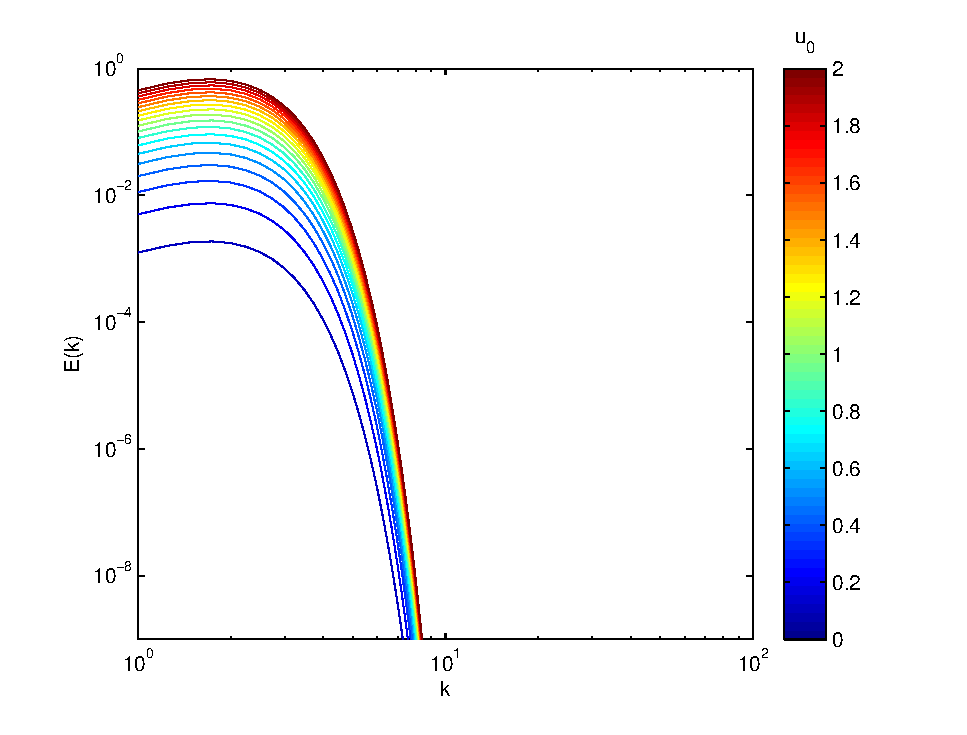
\includegraphics[width=0.48\linewidth]{Figures/eng_spr_u}
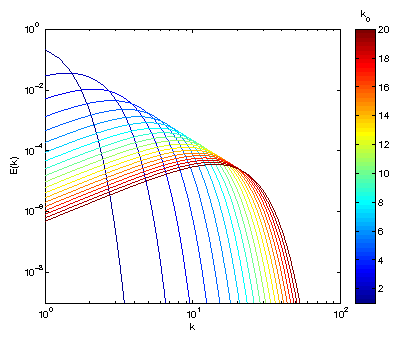
\includegraphics[width=0.48\linewidth]{Figures/eng_spr_k}
\caption{Initial energy spectrum with different parameters: left figure shows the energy spectrum with fixed $k_0 = 2.4$ while varing $u_0$ from $0m/s$ to $2m/s$, right figure shows the one with fixed $u_0 = 0.35m/s$ and varing $k$ from $1$ to $20$.\label{fig:eng_spr}}
\end{figure}

%Following quantities are defined to characterize the turbulence field. 
%The dissipation rate is defined as $\epsilon=2\nu\langle (\nabla\times \mathbf{u})^2)\rangle$,
%$\nu$ is the kinematic viscosity of air $1.5\times10^{-5}m^{2}s^{-1}$, and $u_{rms}$
%is the root mean square of velocity fluctuation. $\tau_{\eta}$ is
%the Kolmogorov time scale defined as $(\nu/\epsilon)^{1/2}$. $\tau_L$
%is the eddy turnover time, estimated by $L_x/u_{rms}$
%where $L_x$ is the domain size.

\begin{figure}[H]\centering
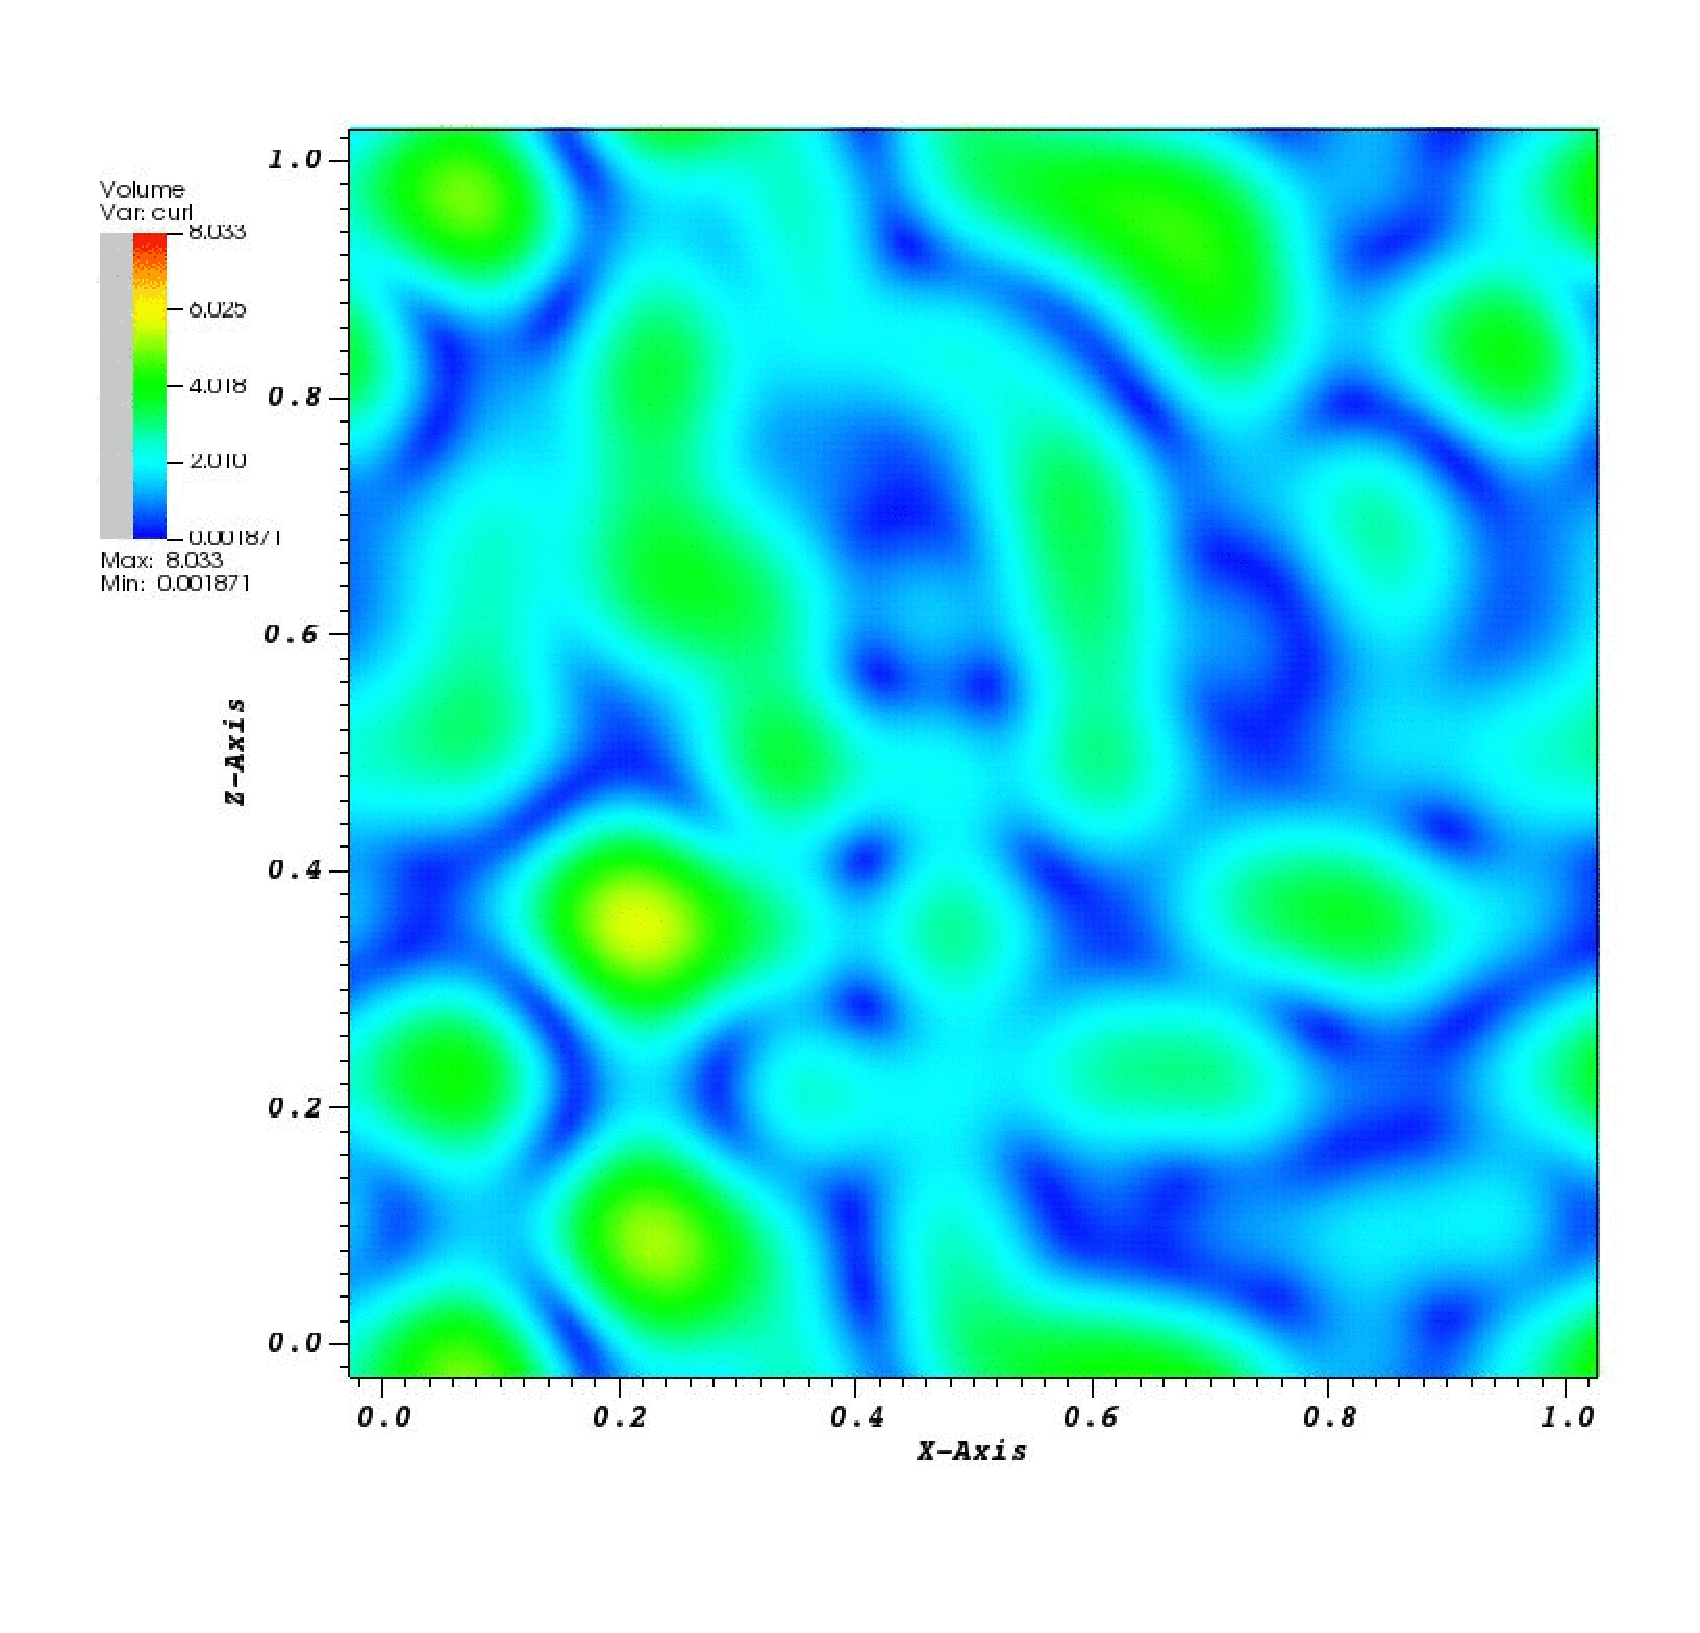
\includegraphics[width=0.48\linewidth]{Figures/vortex-0}
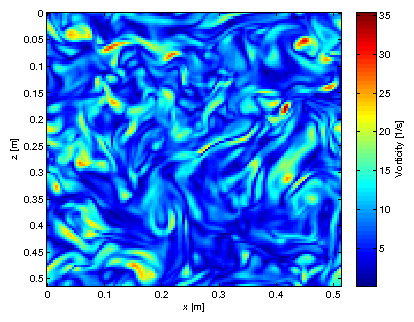
\includegraphics[width=0.48\linewidth]{Figures/vortex-1}

\caption{initial and final vorticity field ($1/s$) in x-z cross-sectional
plane for forced cases\label{fig:enstrophy}}
\end{figure}

\subsection{Initial fields of vapor mixing ratio and temperature}
Three different initial configurations of cloudy area are used to investigate the impact of cloudy area configuration. Case 1 follows that used in \cite{And04} whereby water mixing ratio is defined according to the sign of the velocity function in physical space such that
\begin{equation}
\mbox{case 1: } q_v(\mathbf{x},t=0) = 
\left\{\begin{array}{lr}
q_v^{max}, & u(\mathbf{x}) > 0\\
q_{v,e}, & u(\mathbf{x}) \le 0
\end{array}\right.\label{case1}
\end{equation}
where $q_v^{max} = 3.95 g/kg$ is the maximum amplitude of $q_v$, which exceeds $q_{v,s}$ by $2\%$, and $q_{v,e} = 0.03g/kg$ is the vapor mixing ratio of the clear air. $u(\mathbf{x})$ is the first component of the fluid velocity. 

In \cite{Kumar11}, the author investigated a slab-like cloud configuration approximated with a smooth function to avoid the Gibbs phenomenon (numerical overshoots at sharp interfaces). Similarly, our Case 2 is designed to study the slab-like configuration but approximiated with a simple discontinuous function given by
\begin{equation}
\mbox{case 2: } q_v(x,t=0) = 
\left\{\begin{array}{lr}
q_v^{max}, & (L-d)/2 \le x < (L+d)/2\\
q_{v,e}, & \mbox{elsewhere}
\end{array}\right.\label{case2}
\end{equation}
where the $q_v^{max}$ and $q_{v,e}$ are the same as in Case 1.
$L$ is the length of computational domain, and $d = L/2$ is the width of the cloud slab.

It is well known that entrainment-mixing processes can also occur near cloud tops, esp., for stratiform clouds \cite{Lu2011, Yum2015}. To mimic the cloud-top entrainment-mixing process, herein we add a new cloud configuration by rotating Case 2 by $90$ degree, and name it Case 3.
\begin{equation}
\mbox{case 3: } q_v(z,t=0) = 
\left\{\begin{array}{lr}
q_v^{max}, & (L-d)/2 \le z < (L+d)/2\\
q_{v,e}, & \mbox{elsewhere}
\end{array}\right.\label{case3}
\end{equation}

The temperature field is initialized by imposing the neutral buoyancy condition \cite{Kumar14} such that:
\begin{equation}
T(x,t = 0) = T_0 - 0.608T_0[q_v(x,t = 0) - q_{v0}]
\end{equation}
where the reference values are defined by the domain averages $T_0 = \langle T(t=0)\rangle_V$ and $q_{v0} = \langle q_v(t=0)\rangle_V$. This neutral buoyancy condition ensures the initial cloudy area having higher water vapor mixing ratio but lower temperature compared to the environment. Note that this procedure is only performed for the initial temperature field; later temperature field completely follow \Eq{eq:Temp} afterwards. \Fig{fig:slice_case123} compares the initial fields of water vapor 
mixing ratio and temperature for the three cases. The discrepancies between the initial water vapor 
and temperature fields are self-evident, allowing for examination of the impacts of the initial 
configuration of cloudy area on entrainment-mixing processes. Note that all the three initial 
configurations have the same initial cloud fraction of $0.5$, and the same dynamical field.

\begin{figure*}\centering
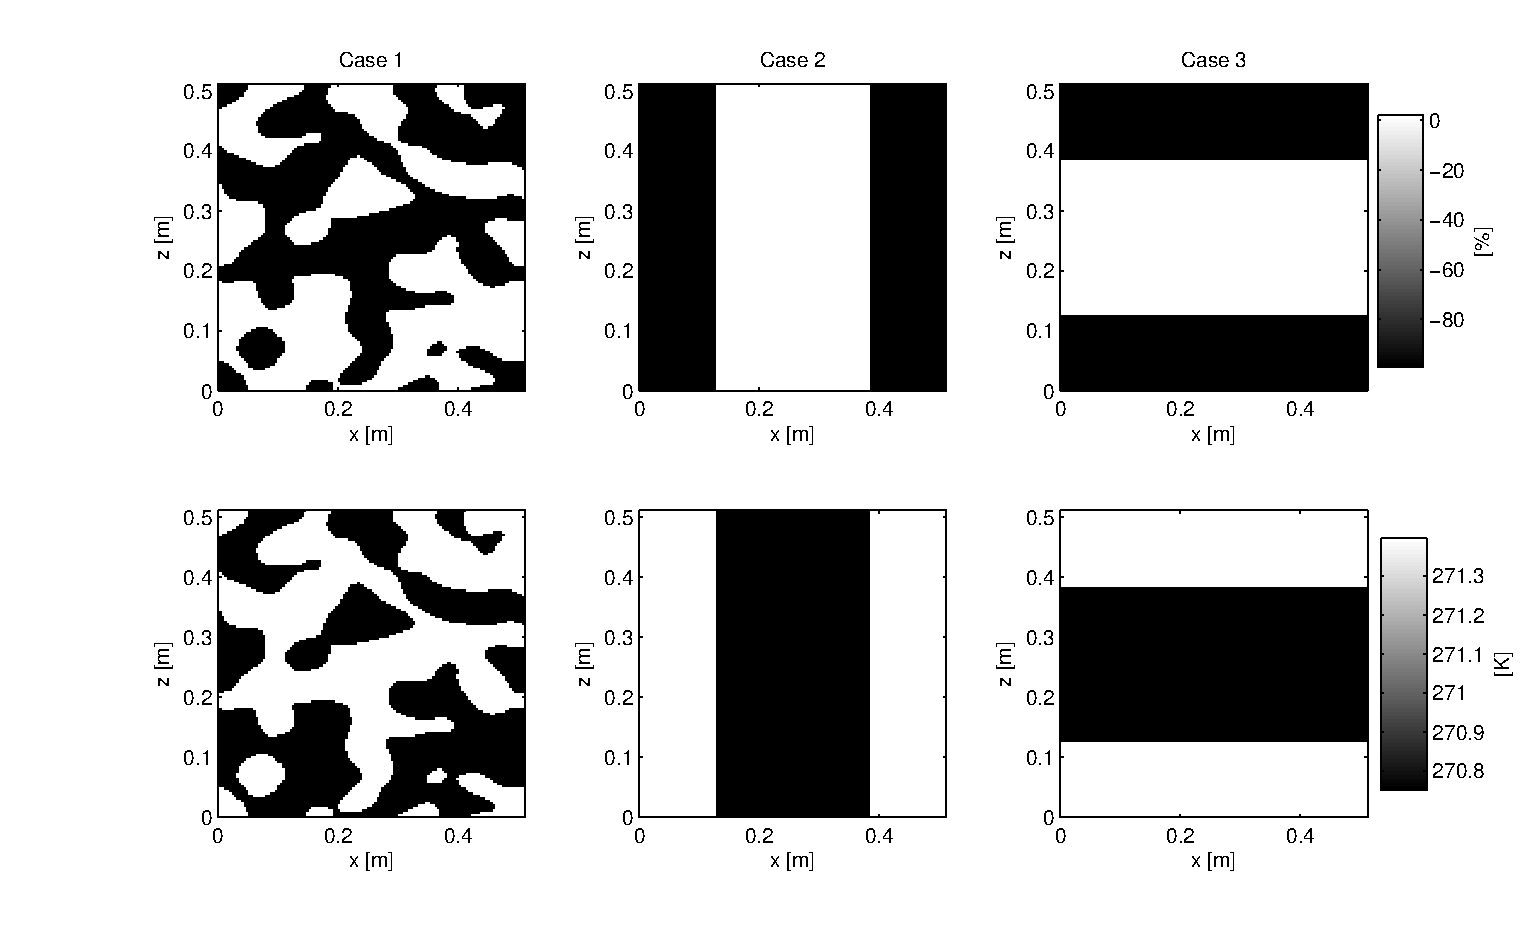
\includegraphics[width=0.9\linewidth]{Figures/init_vapor_supersat}
\caption{Cross sectional view of the initial supersaturation and temperature (K) field for different cases: case 1, 2, 3 from left to right. The cloudy part occupies about half of the computational domain.\label{fig:slice_case123}}
\end{figure*}

\subsection{Initial droplets}

At beginning, a total of $10^{7}$ droplets with the same radius of $15\mu m$  are randomly placed in the cloudy area according to the Poisson point process, giving a droplet number concentration of $ ~ 153{cm}^{-3}$. Note that for the forced turbulence scenario, the velocity field needs a few steps ($5$ seconds here) to relax to a steady state. Therefore, the droplets are released to move and change their sizes according to the physics law after this spin-up period. For the decaying turbulence, the droplets are released at time $t = 0s$ since there is no needs to seek for a steady state. The simulation is terminated when droplets completely evaporate or the field becomes nearly uniform ($std < 0.0002$). 

For convenience, \Table{tb:parameters} summarizes the key quantities and initial conditions.
\begin{table*}[T]
\begin{tabular}{l c c c c c}
\hline\hline
Quantity & Symbol & Value & Quantity & Symbol & Value\\
\hline
Grid points & $N$ & $256$ & Droplet radius & $R_{0}$ & $15\mu m$\\
Box length & $L$ & $0.512m$ & Environ supersat & $S_{e}$ & $-99\%$\\
Grid size & $a$ & $0.002m$ & Cloud supersat & $S_{c}$ & $2\%$\\
Viscosity & $\nu$ & $1.5\times10^{-5}m^{2}s^{-1}$ & Number concentration& $N_{c}$ & $153cm^{-3}$\\
Dissip rate& $\epsilon$ & $2.0\times10^{-3}m^{2}s^{-3}$ & Eddy turnover time & $\tau_{L}$ & $4.27s$\\
Dissip length& $\eta$ & $10^{-3}m$ & Evaporation time & $\tau_{evap}$ & $2.09s$\\
Dissip time& $\tau_{\eta}$ & $0.087s$ & Reaction time & $\tau_{react}$ & $4.52s$\\
\hline
\end{tabular}
\caption{Summary of key model parameters and initial conditions}
\label{tb:parameters}
\end{table*}

\section{Numerical Results}\label{numerical_results}
Six numerical experiments are performed to represent six scenarios (denoted by D1, D2, D3, F1, F2, and F3) according to the combination of the two different turbulence setups (decaying vs forced) and three different initial configurations of cloudy area (Case 1, Case2, and Case 3). This section presents the results, with a focus on entrainment-mixing processes. 

\subsection{Evolution of dynamical and thermodynamic fields}
\Fig{fig:therm_dynam} compares the temporal evolutions of the domain mean, standard deviation and relative dispersion of turbulent kinetic energy (TKE, a, b, c), of temperature (d,e,f) and water vapor mixing ratio (g, h, i), and supersaturation (j, k, l) between the six scenarios.  As expected, the mean TKE and its standard deviation for the three forced simulations (F1, F2 and F3) remain approximately constant determined by the large scale forcing after a short relaxation at the initial time. However, it is interesting to observe a transient turbulence enhancement before gradually decaying to zero in the decaying cases, especially for D2 and D3. This transient enhancement likely results from the buoyancy effect, which is caused by the deviation of temperature and vapor mixing ratio to the reference value according to \Eq{eq:source_term}. The D3 simulation exhibits the strongest enhancement, followed by D2. But for D2 the enhancement lasts longer. The mixing in D3 is accelerated by the sedimentation effect, making it a slightly stronger and faster than D2. Note that D1 can be regarded as the intermediate stage of mixing process in D2 or D3, and therefore the buoyancy effect quickly disappear and show little enhancement in the figure.  Most of the droplets have a chance to enter into the clear air and evaporate at an early stage. Evaporation process absorbs latent heat from the environment, resulting in deviation of the temperature field from the mean value. The transient enhancement can be seen more clearly from the standard deviation of temperature. The transient enhancement is weaker for the three forced simulations F1, F2 and F3 (but still stronger than that of TKE).  It is noteworthy that the behavior of transient turbulence enhancement does not appear in the field of water vapor mixing ratio, which is consistent with \cite{Kumar14}. Notice that the vapor mixing ratio in the clear air is much lower than in the cloudy air. The droplets entering into the clear area will quickly turn into vapor while the droplets staying in the cloudy area continue to grow by condensation. This phase transition process reduces the difference of vapor mixing ratio between clear air and cloudy air, thus the transient growth of the deviation can hardly be observed.  The behavior of supersaturation reflects the combination of temperature and water vapor mixing ratio, as expected. The variations manifest themselves in the plots of relative dispersion defined as standard deviation to the mean of the corresponding variables.

\begin{figure*}[!htbp]\centering
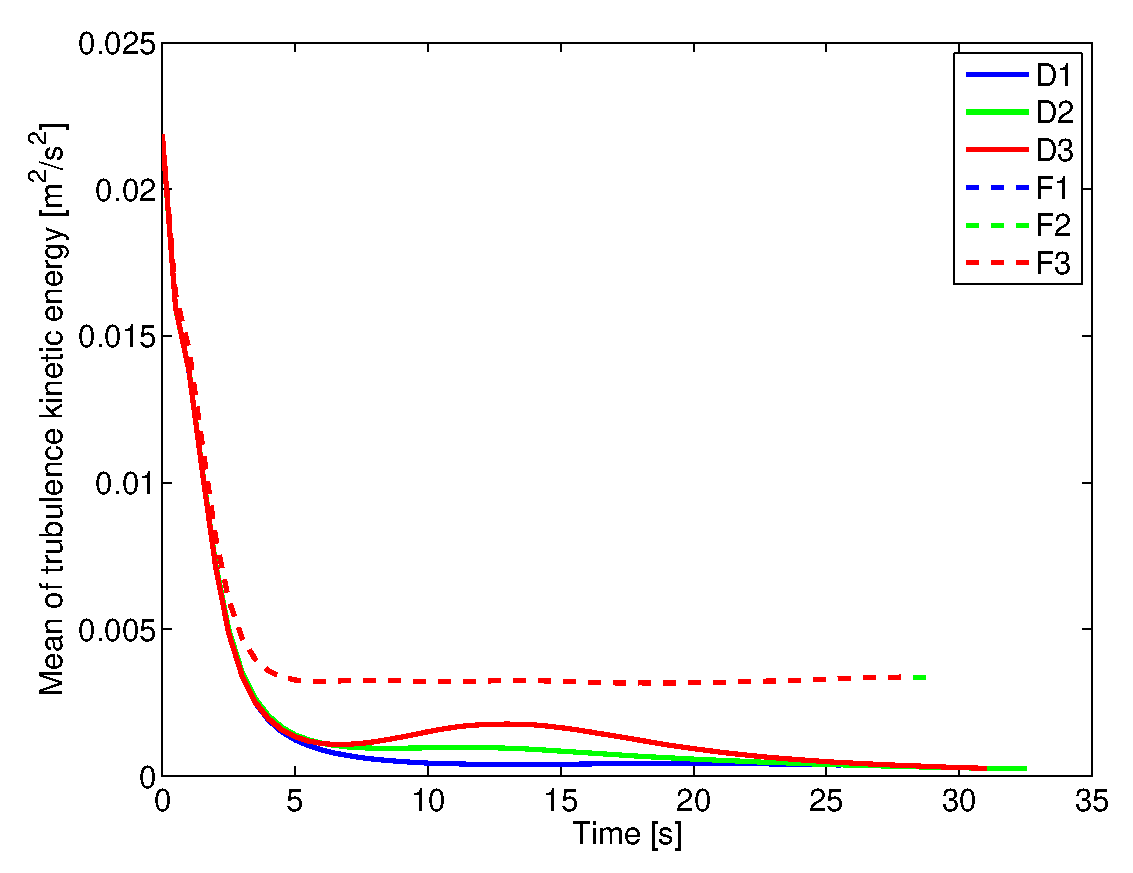
\includegraphics[width=0.3\linewidth]{Figures/mean_tke}
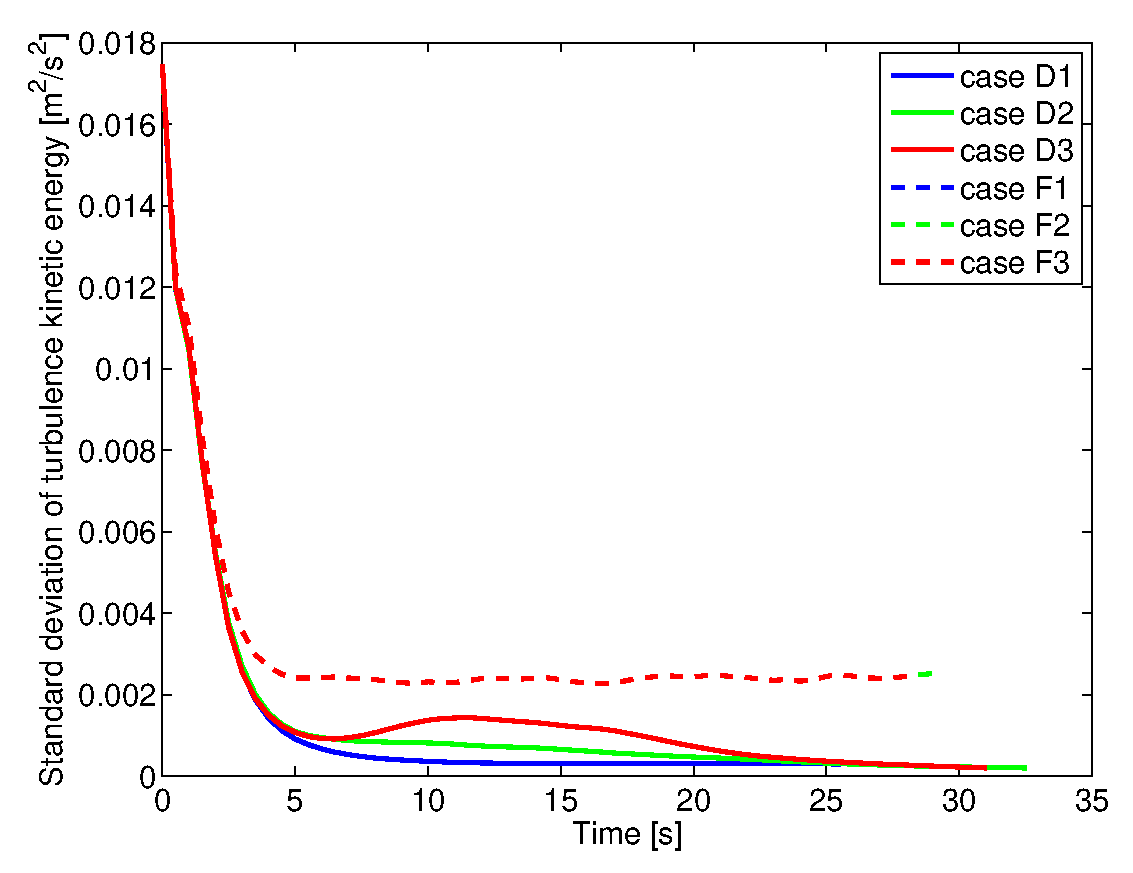
\includegraphics[width=0.3\linewidth]{Figures/std_tke}
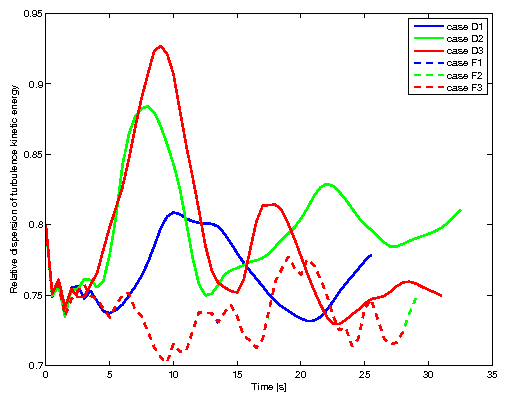
\includegraphics[width=0.3\linewidth]{Figures/dsp_tke}\\
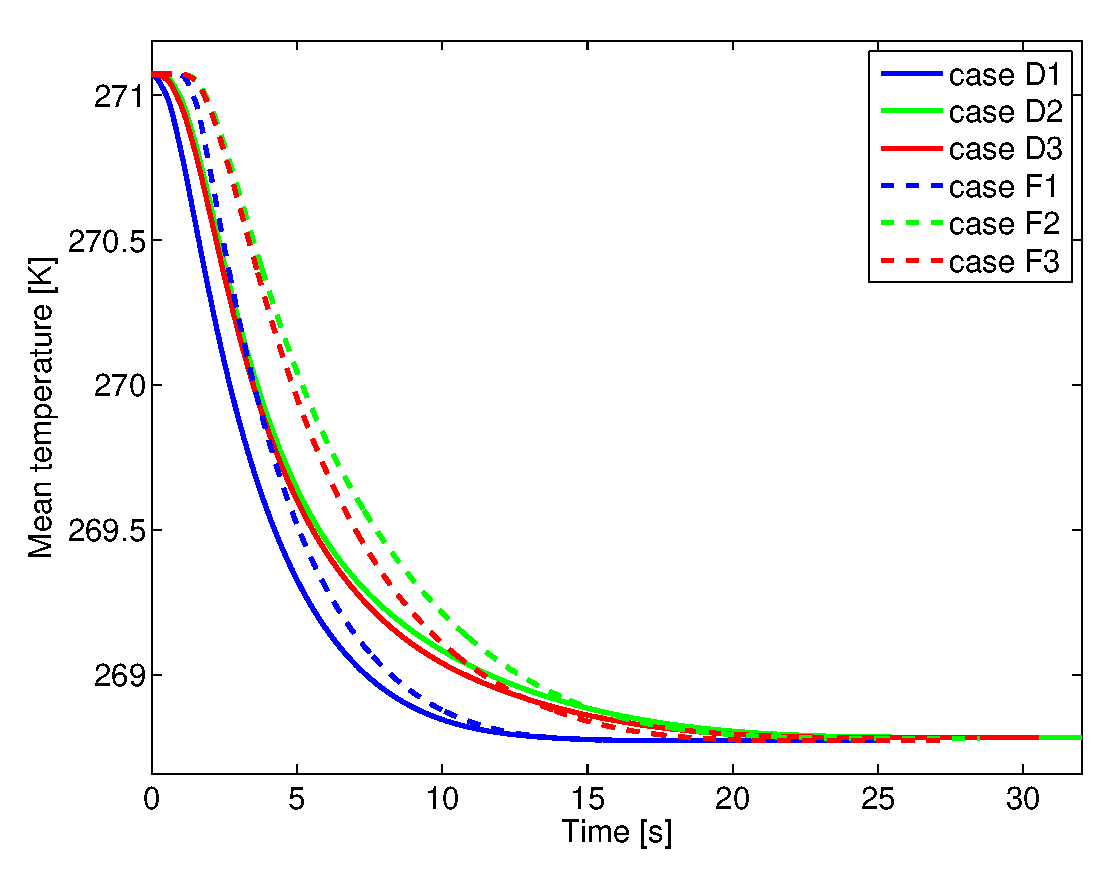
\includegraphics[width=0.3\linewidth]{Figures/mean_temp}
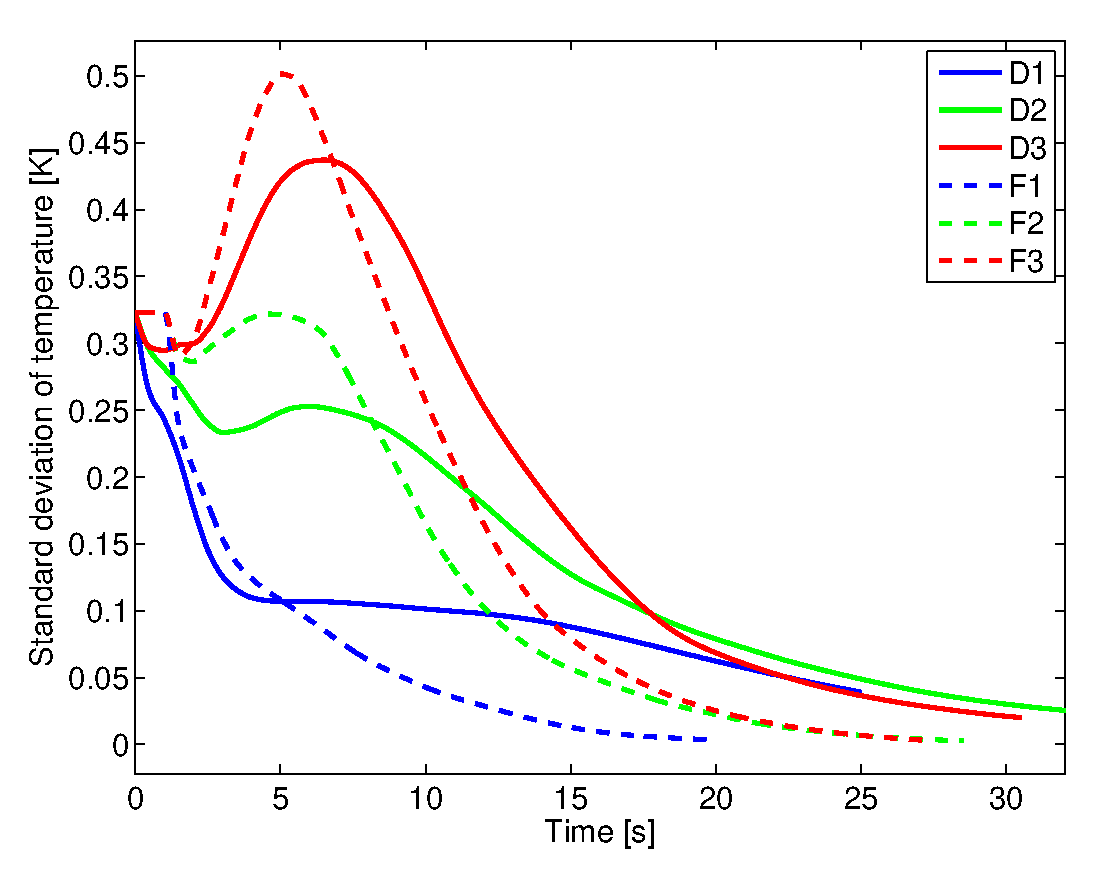
\includegraphics[width=0.3\linewidth]{Figures/std_temp}
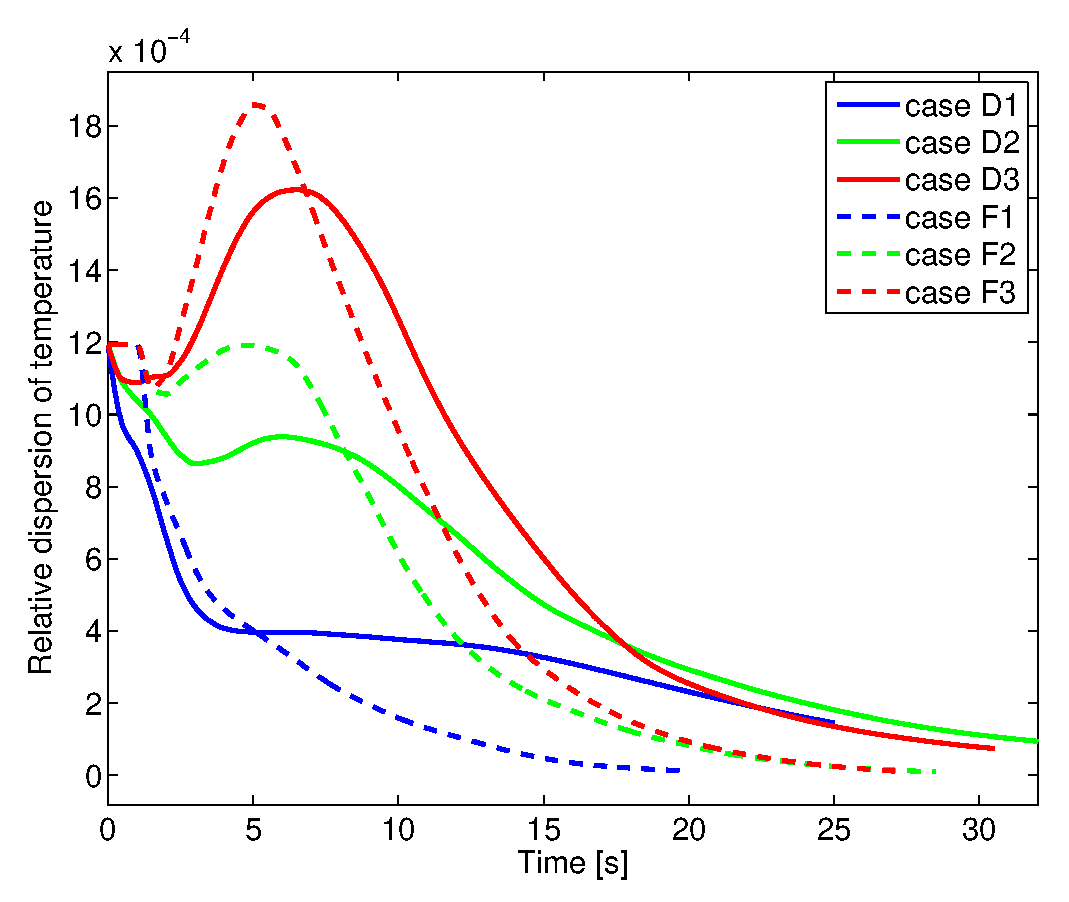
\includegraphics[width=0.3\linewidth]{Figures/dsp_temp}\\
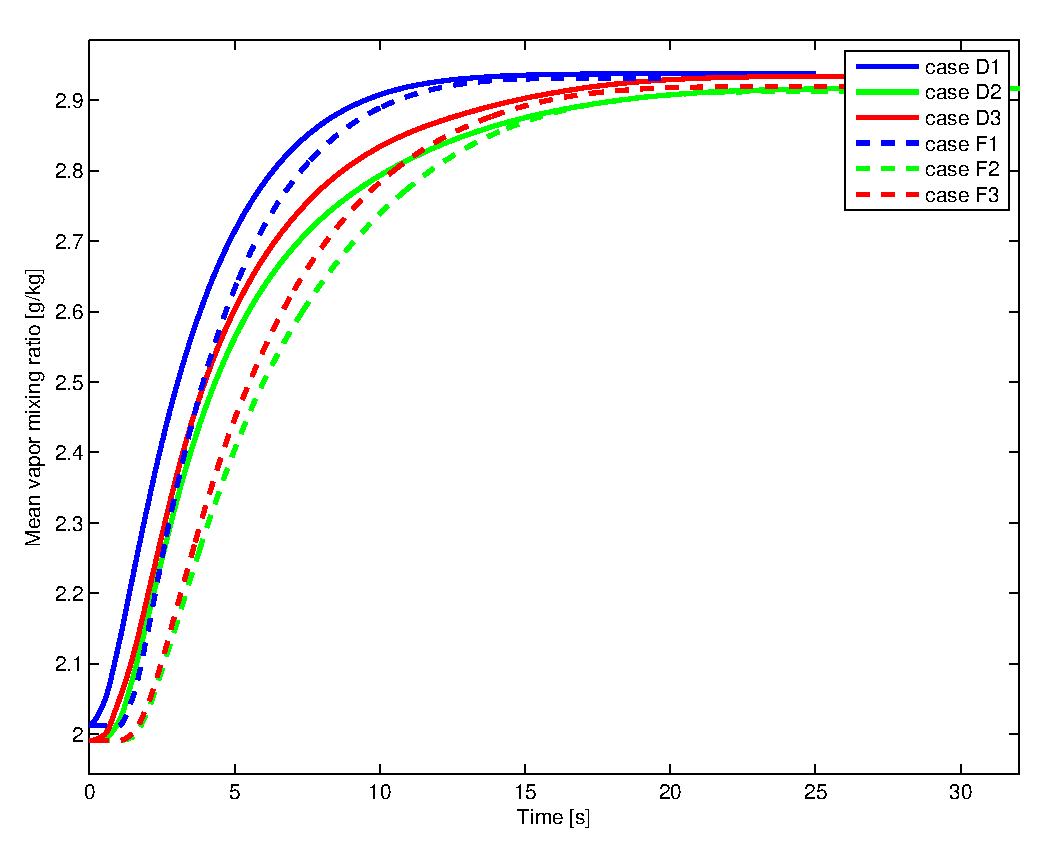
\includegraphics[width=0.3\linewidth]{Figures/mean_vapor}
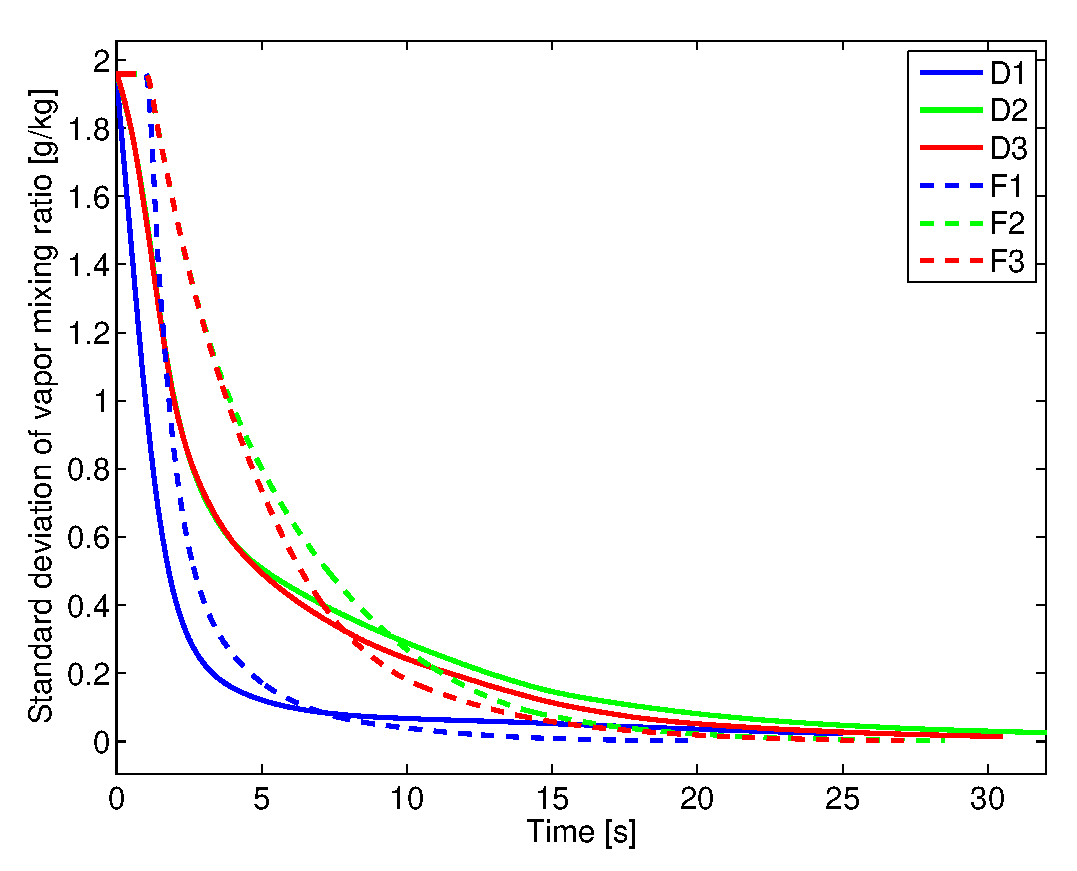
\includegraphics[width=0.3\linewidth]{Figures/std_vapor}
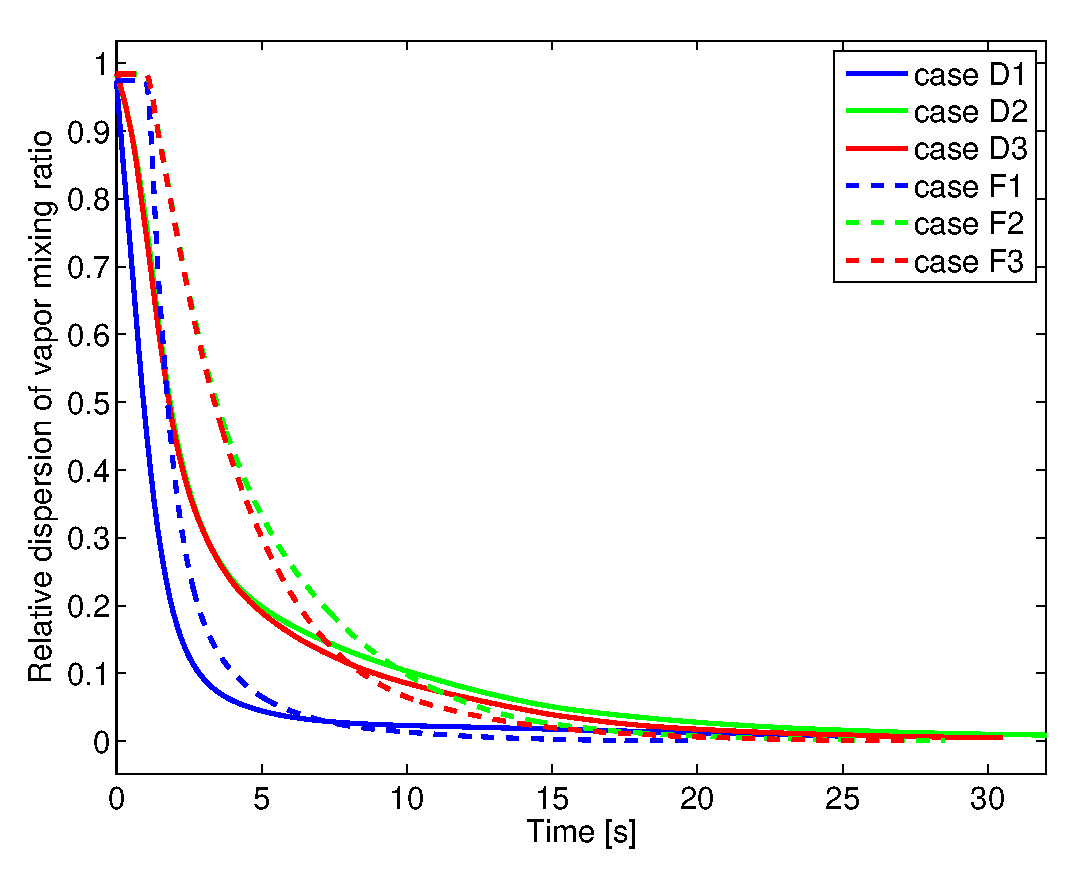
\includegraphics[width=0.3\linewidth]{Figures/dsp_vapor}\\
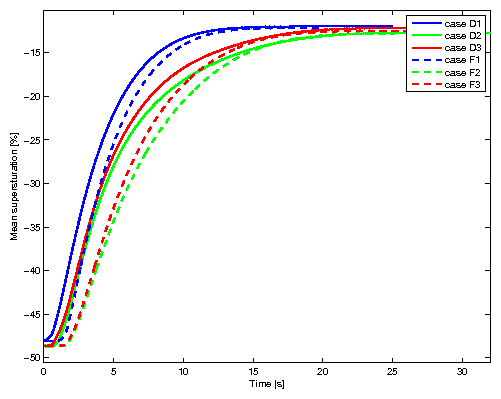
\includegraphics[width=0.3\linewidth]{Figures/mean_super}
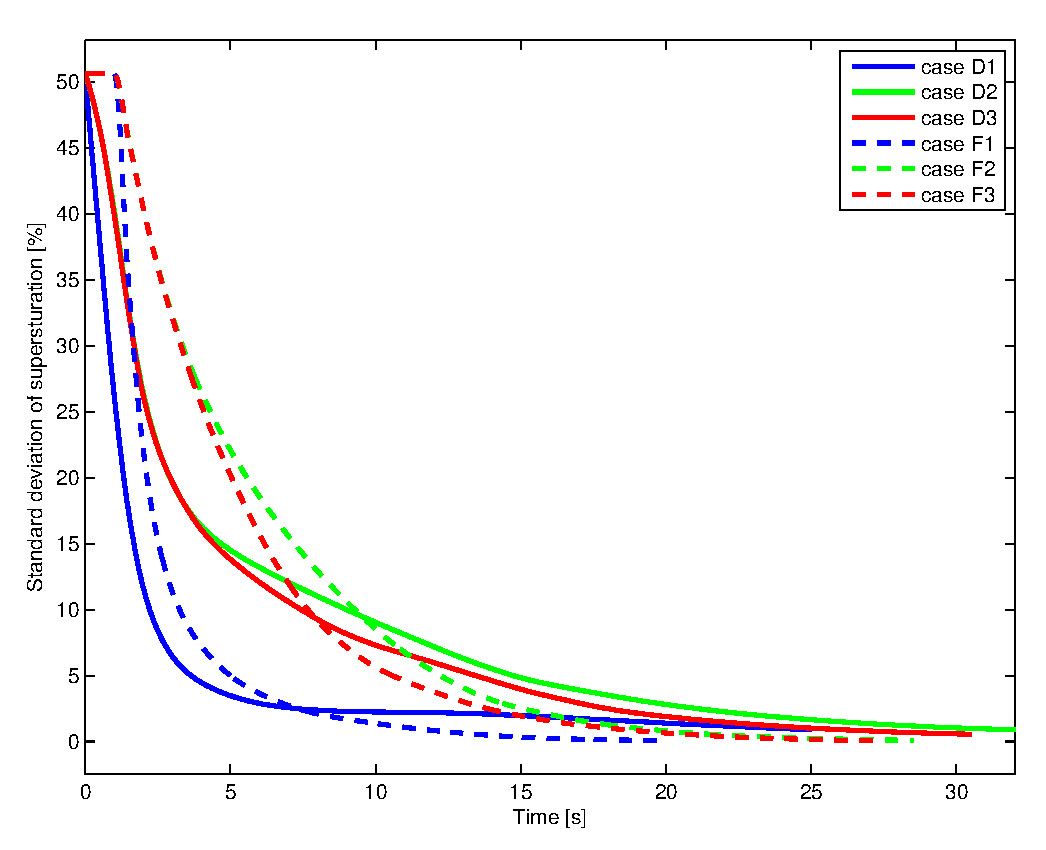
\includegraphics[width=0.3\linewidth]{Figures/std_super}
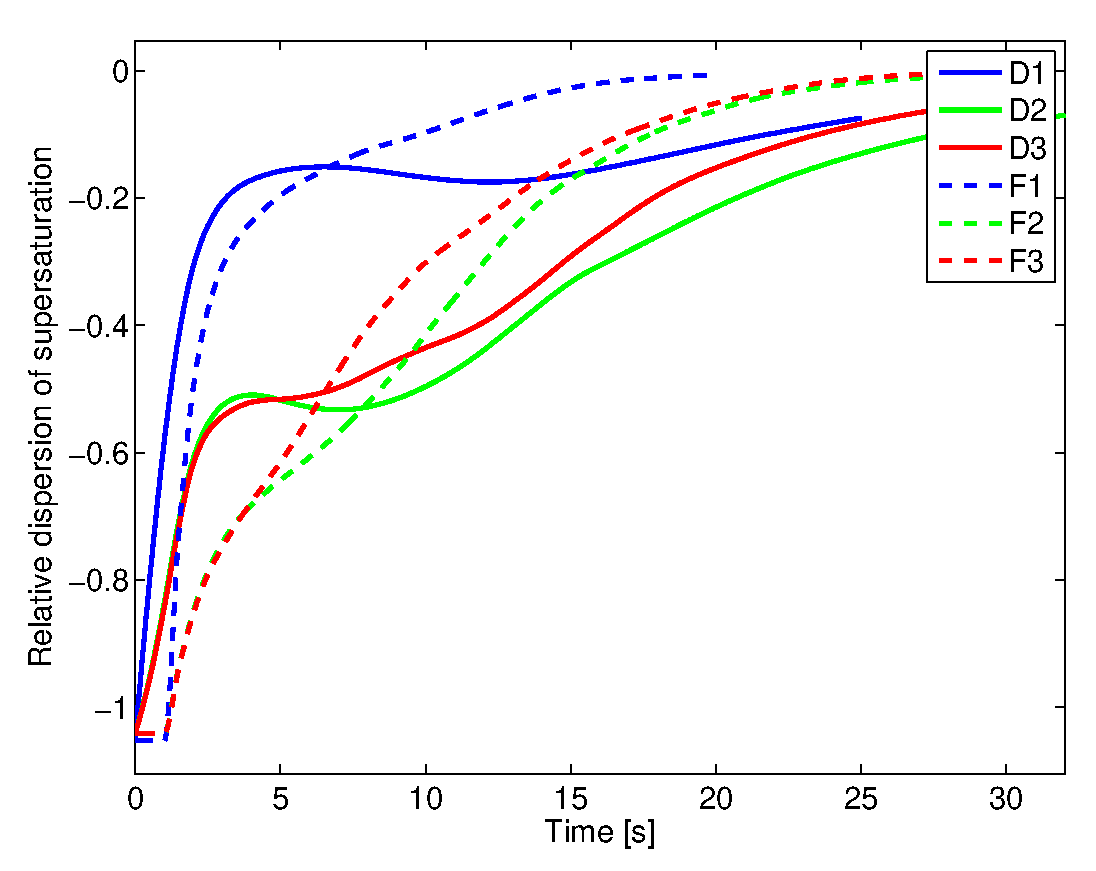
\includegraphics[width=0.3\linewidth]{Figures/dsp_super}
\caption{Thermodynamics of three cases. The left column is the mean value, middle column is the standard deviation and left column is the relative dispersion defined as the ratio of standard deviation and mean. The rows from top to bottom are turbulent kinetic energy, temperature, vapor mixing ratio and supersaturation.\label{fig:therm_dynam}}
\end{figure*}

\subsection{Microphysics}
\Fig{fig:rad_distri} shows temporal variation of the cloud droplet size distribution for all the six simulations. A few points are evident. First, the droplet size distributions start with a monodisperse distribution with a uniform droplet radius of $15\mu m$. As the turbulent mixing between the subsaturated environment and the supersaturated cloudy air proceeds, some droplets evaporate, the size distributions gradually shift to small sizes and broadens until all droplets completely evaporate or the background environment become saturated. Due to the initial configuration, the final states of all the cases contain no droplets and result in unsaturated environments. Second, the three cases with decaying turbulence (D1, D2 and D3) are quite different in their evolutions of size distributions. However, the difference between the three forced turbulence cases (F1, F2 and F3) almost disappear, demonstrating that the buoyancy effect is overwhelmed by the external forcing and the differences in the decaying cases are caused by the buoyancy term in \Eq{eq:source_term}. The role of buoyancy in broadening is also evident from the comparison of the corresponding simulations with decaying and forced turbulence.
\begin{figure}[!htbp]\centering
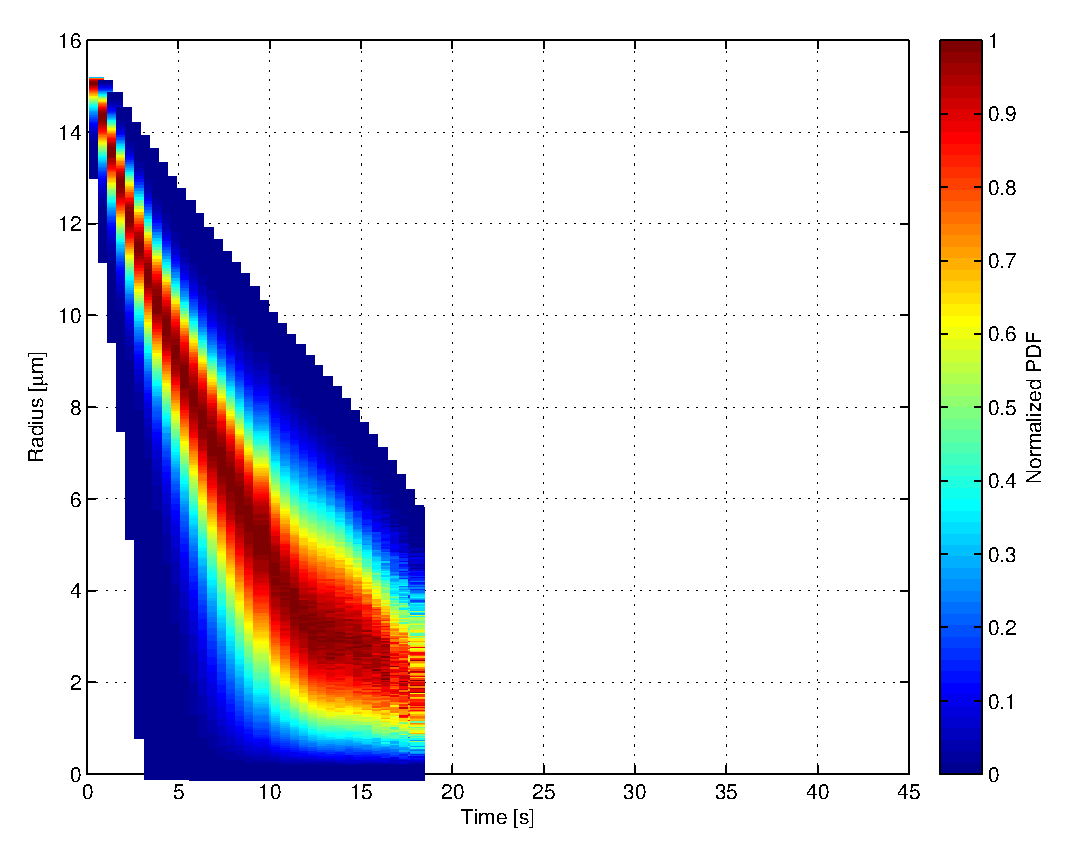
\includegraphics[width=0.48\linewidth]{Figures/pdf_radius_d1}
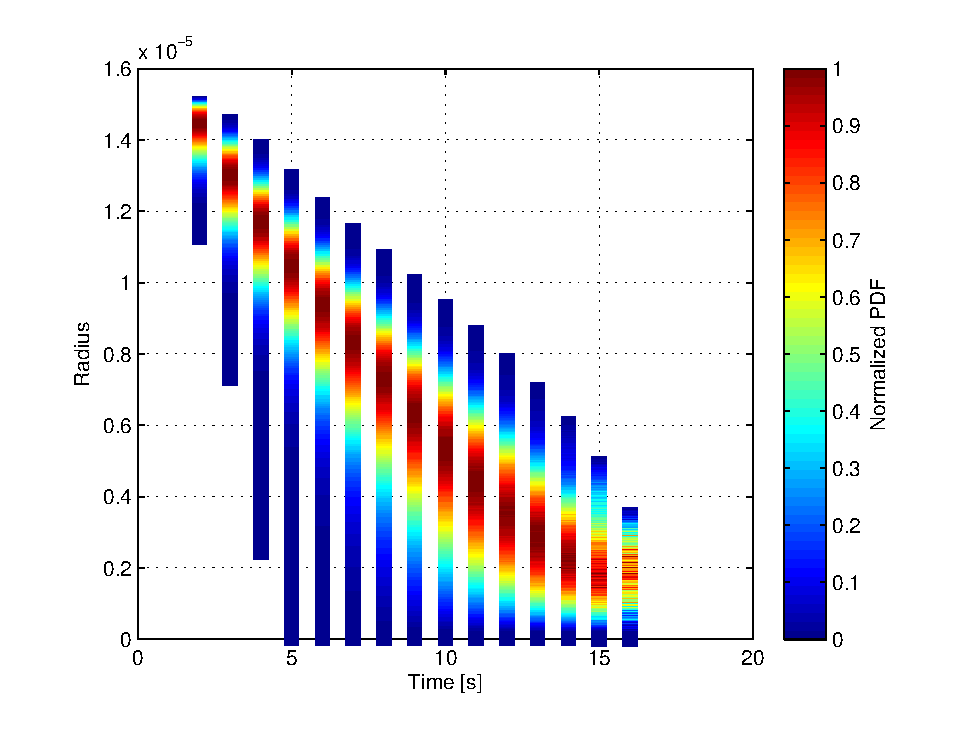
\includegraphics[width=0.48\linewidth]{Figures/pdf_radius_f1}\\
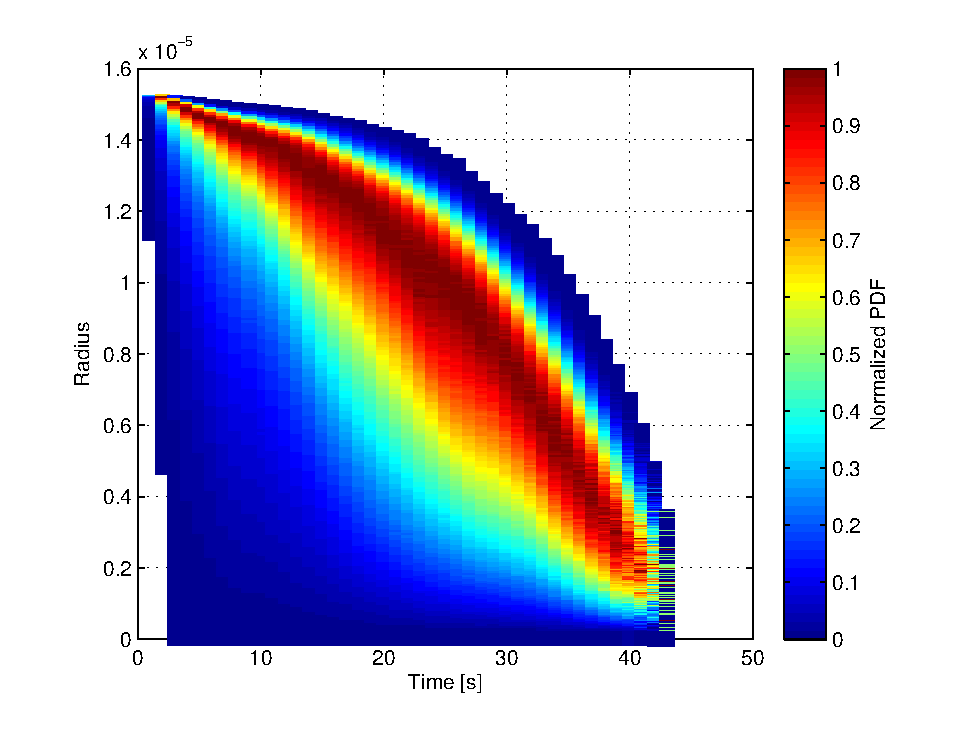
\includegraphics[width=0.48\linewidth]{Figures/pdf_radius_d2}
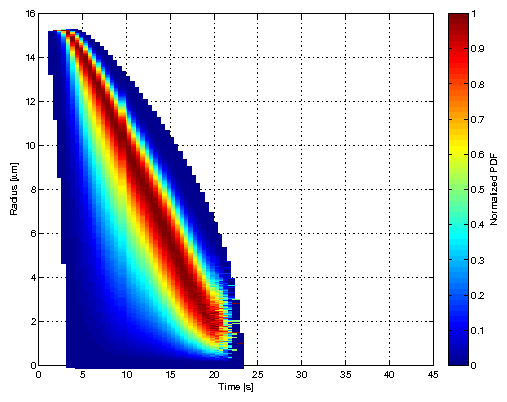
\includegraphics[width=0.48\linewidth]{Figures/pdf_radius_f2}\\
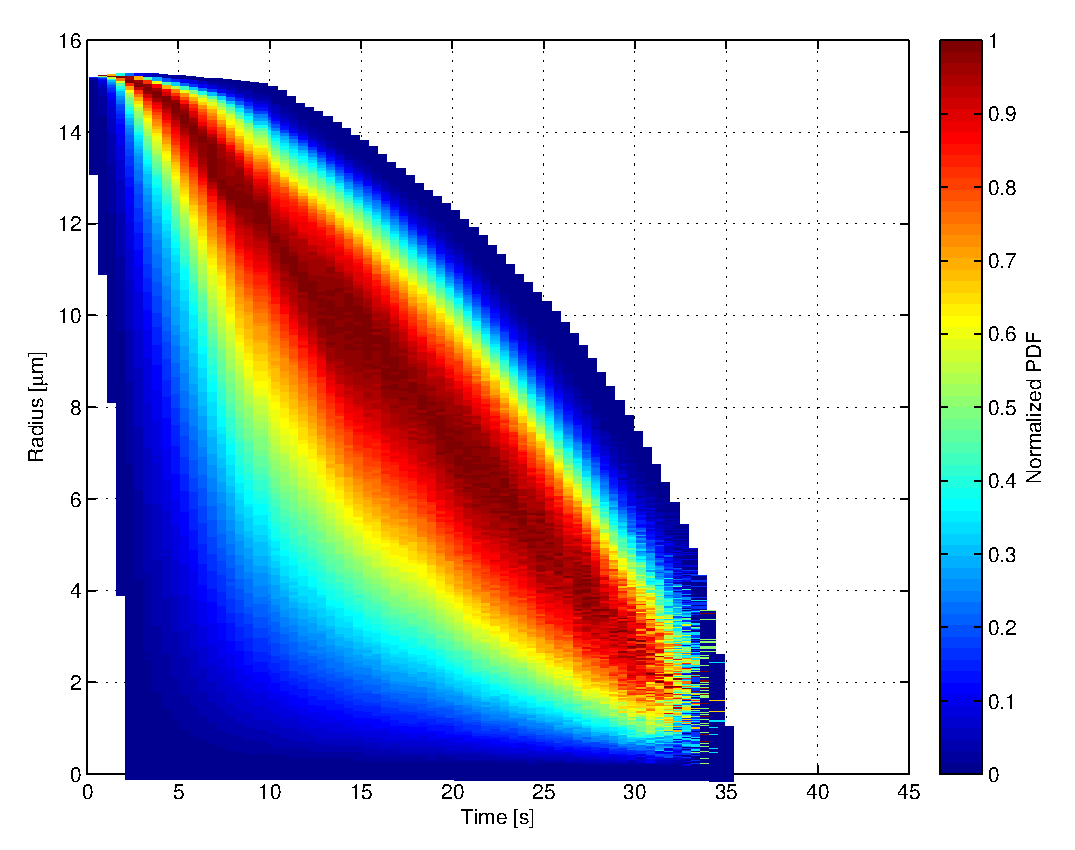
\includegraphics[width=0.48\linewidth]{Figures/pdf_radius_d3}
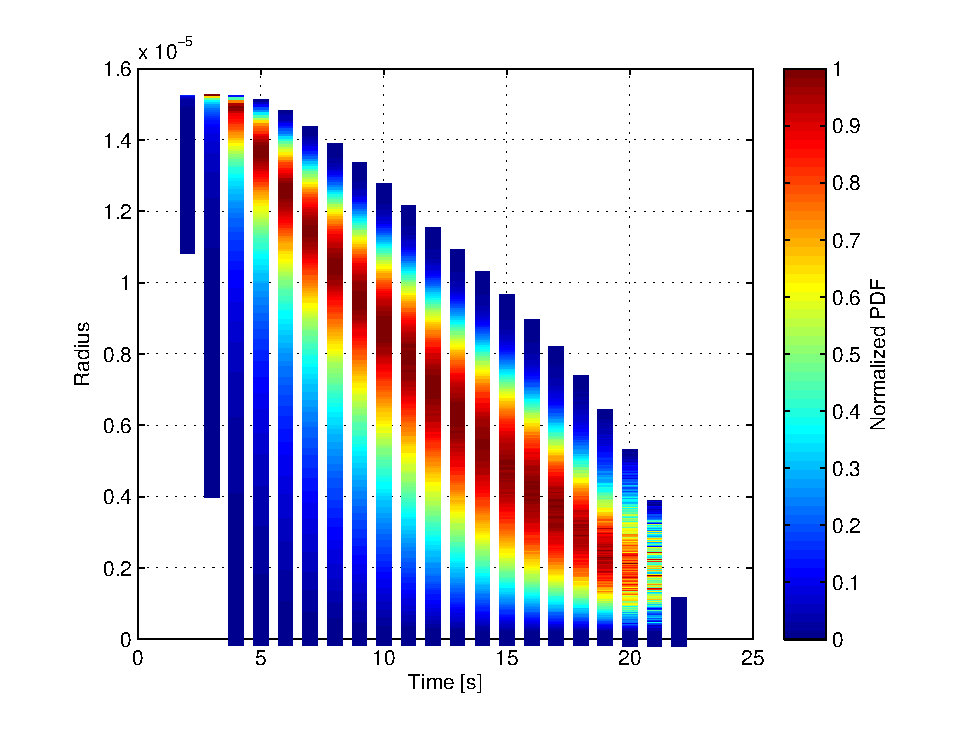
\includegraphics[width=0.48\linewidth]{Figures/pdf_radius_f3}
\caption{Evolution of radius distribution for decaying turbulence (left column) 
and forced turbulence (right column). From up to bottom are case 1, case 2 and case 3 respectively.}\label{fig:rad_distri}
\end{figure}

To better illustrate the impacts of different simulation scenarios, \Fig{fig:temporal_variation} shows the temporal evolution of the domain-mean liquid water content (a), droplets concentration (b), 
mean volume radius (c), mean radius (d), standard deviation (e) and relative dispersion (f). Several points are evident. First, in all the simulations, LWC and droplet concentration decrease as turbulent mixing and droplet evaporation proceed. The mean volume radius and mean radius also decreases with time because the decrease of liquid water content is stronger/faster than that of droplet concentration. Second, in all the simulations, standard deviations first increase, peak at some time, and then decrease beyond the peak time. The occurrence of maximum standard deviation steps from the combined spectral broadening related to entrainment-mixing processes and the shrinking of droplet populations due to evaporation. Also noteworthy is that the peak standard deviations occur between $x$ and $y$ for all the six simulation scenarios. The coupled variations of mean radius and standard deviation result in relative dispersion peaks at a much later time compared to standard deviation. Finally, despite the commonalities, the differences among the different scenarios are evident. Since the configuration of Case 1 is close to an already-mixed case, its number concentration and mean radius decay at a faster rate, and the standard deviation of the droplet size is lower than other cases. Case 2 and Case 3 have no big difference except the number concentration. Since the mixing process of Case 3 is accelerated by the buoyancy effects in the vertical direction, the number concentration of Case 3 has a stronger decrease than Case 2. Comparing the forced cases and decaying cases, at least two phases can be observed. In the first stage, the forced cases contain more liquid water content, larger number concentration and mean radius than the corresponding decaying cases, while exhibit an opposite result in the later stage. This implies that the decaying cases initially have faster mixing and evaporation while are overtaken by the forced turbulence later. 
  
\begin{figure}[!htbp]\centering
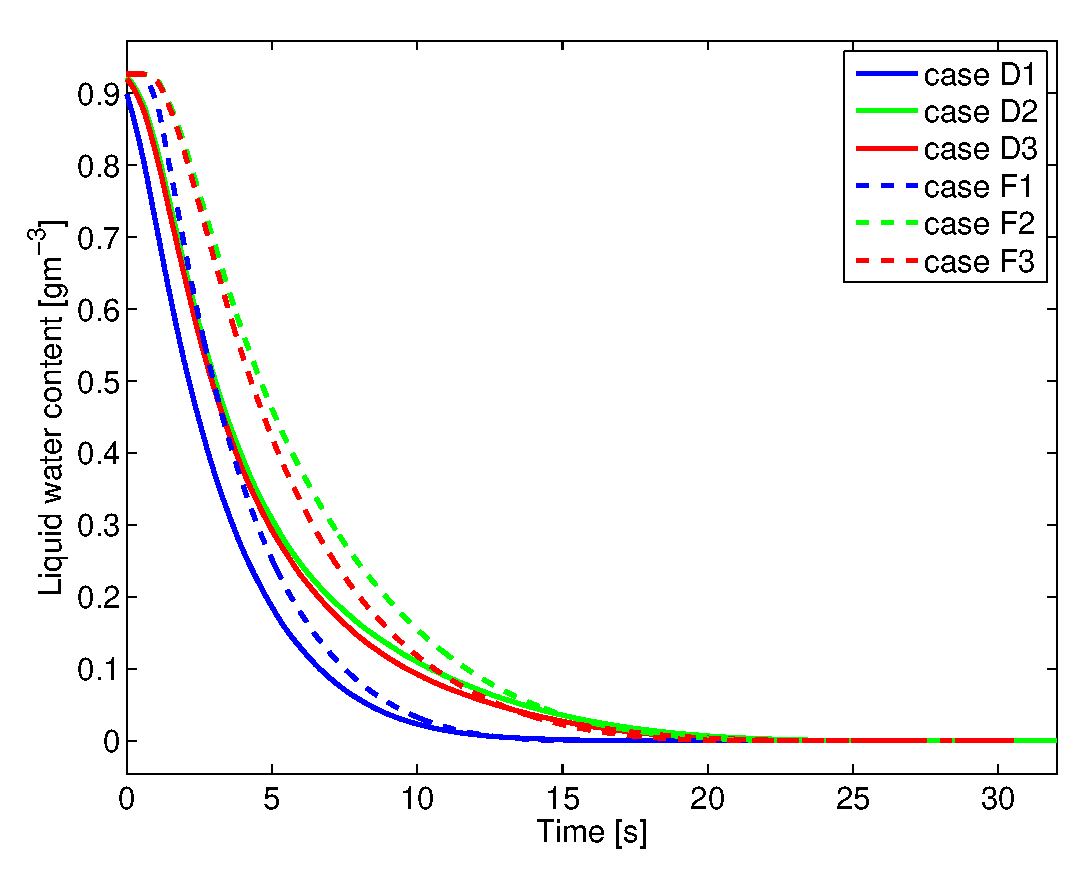
\includegraphics[width=0.48\linewidth]{Figures/lwc}
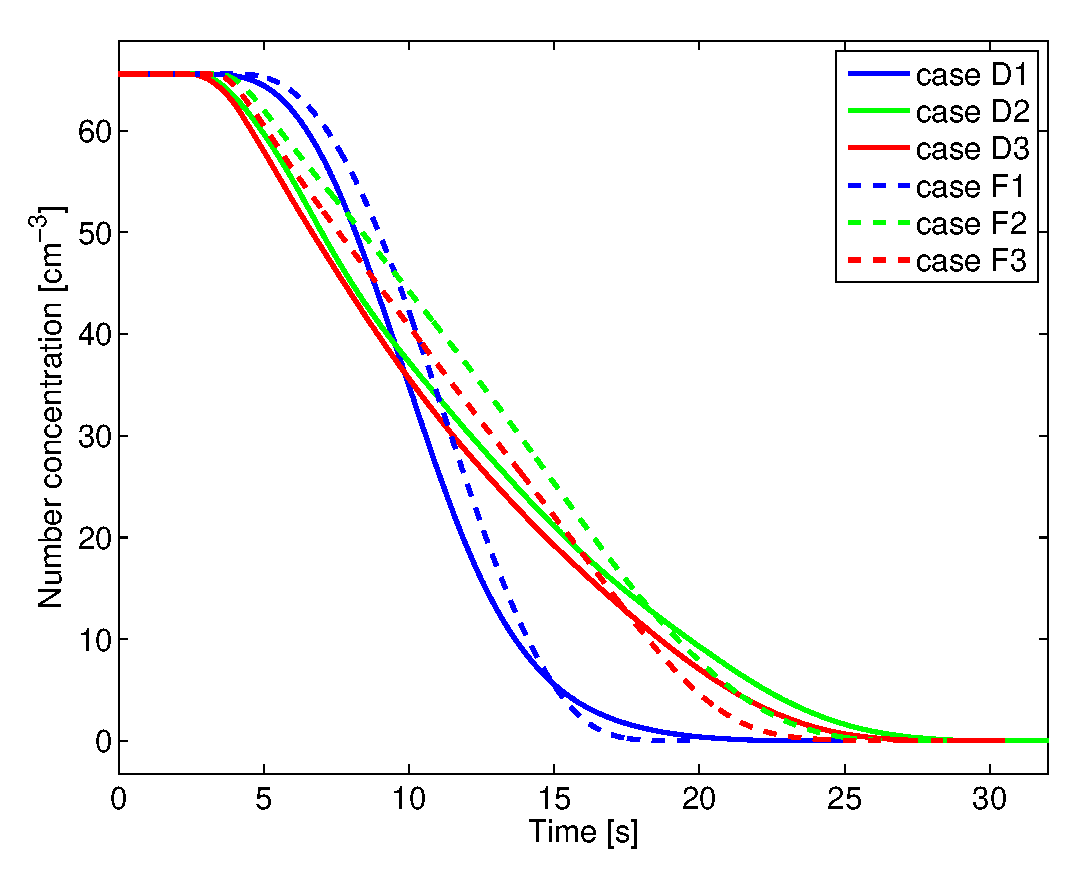
\includegraphics[width=0.48\linewidth]{Figures/num_con}\\
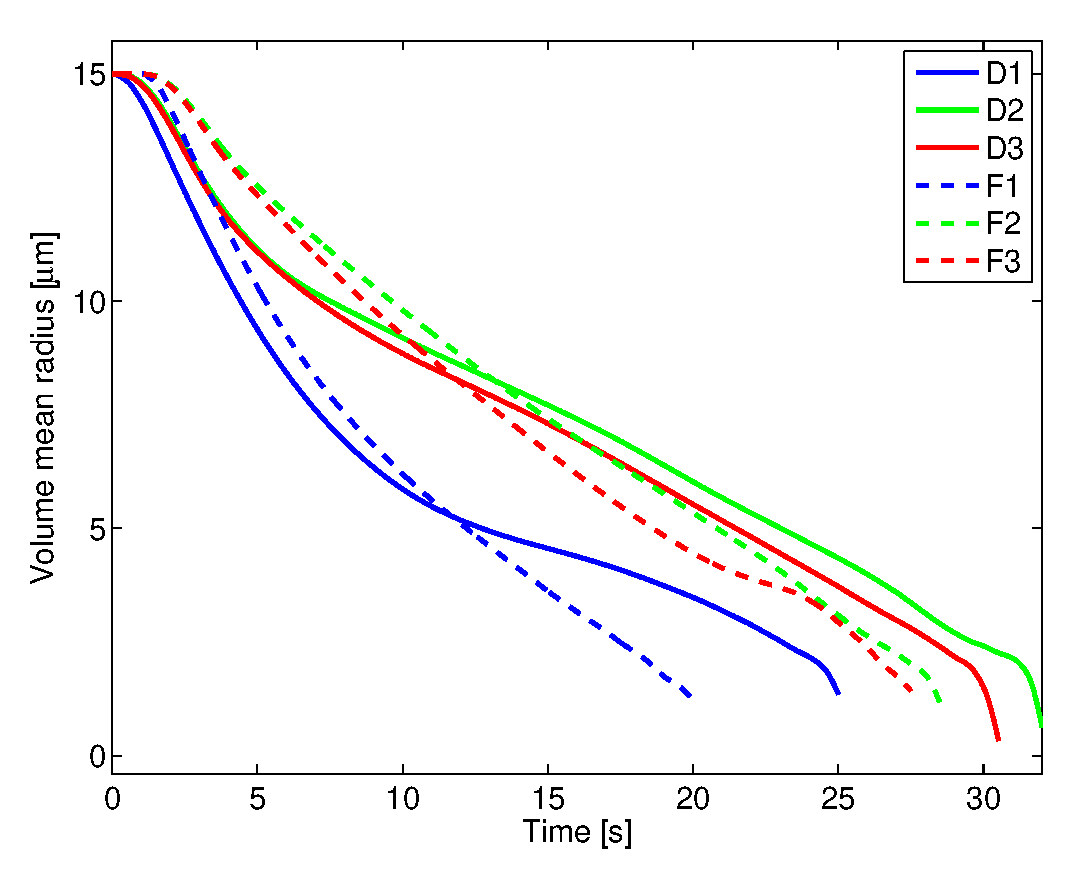
\includegraphics[width=0.48\linewidth]{Figures/vmean_radius}
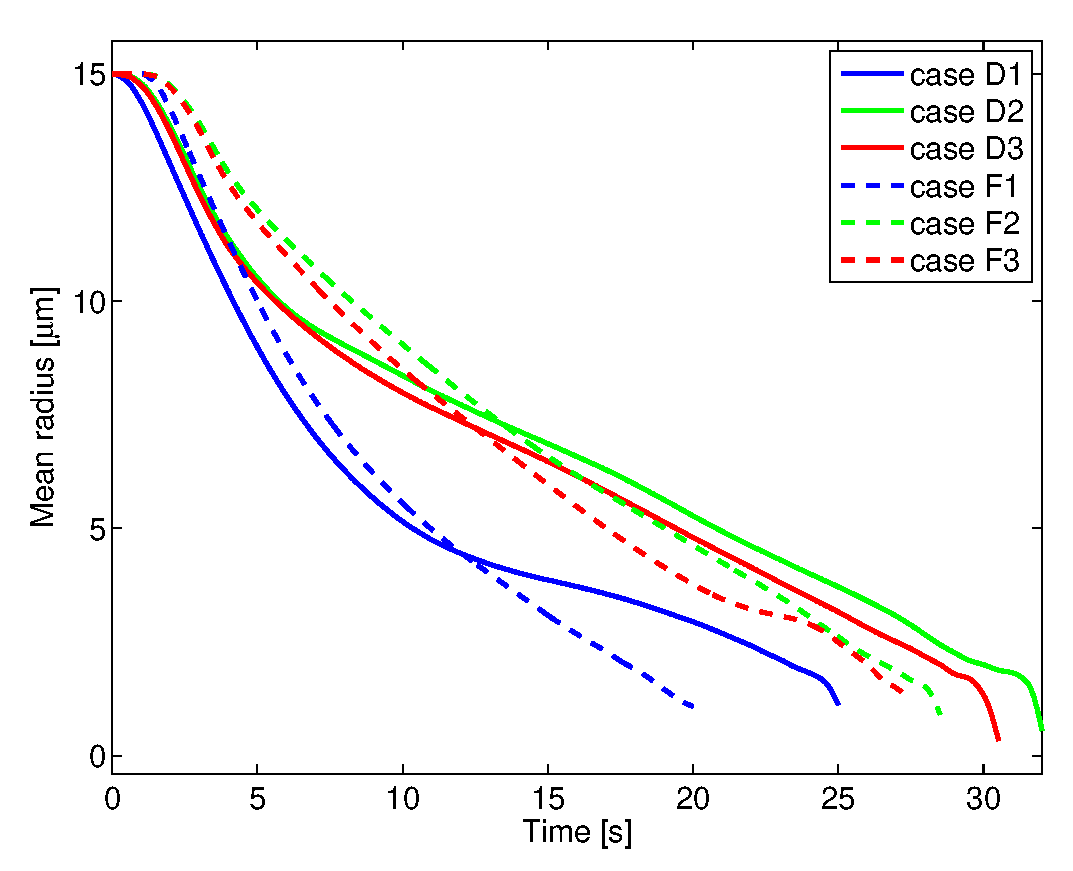
\includegraphics[width=0.48\linewidth]{Figures/mean_radius}\\
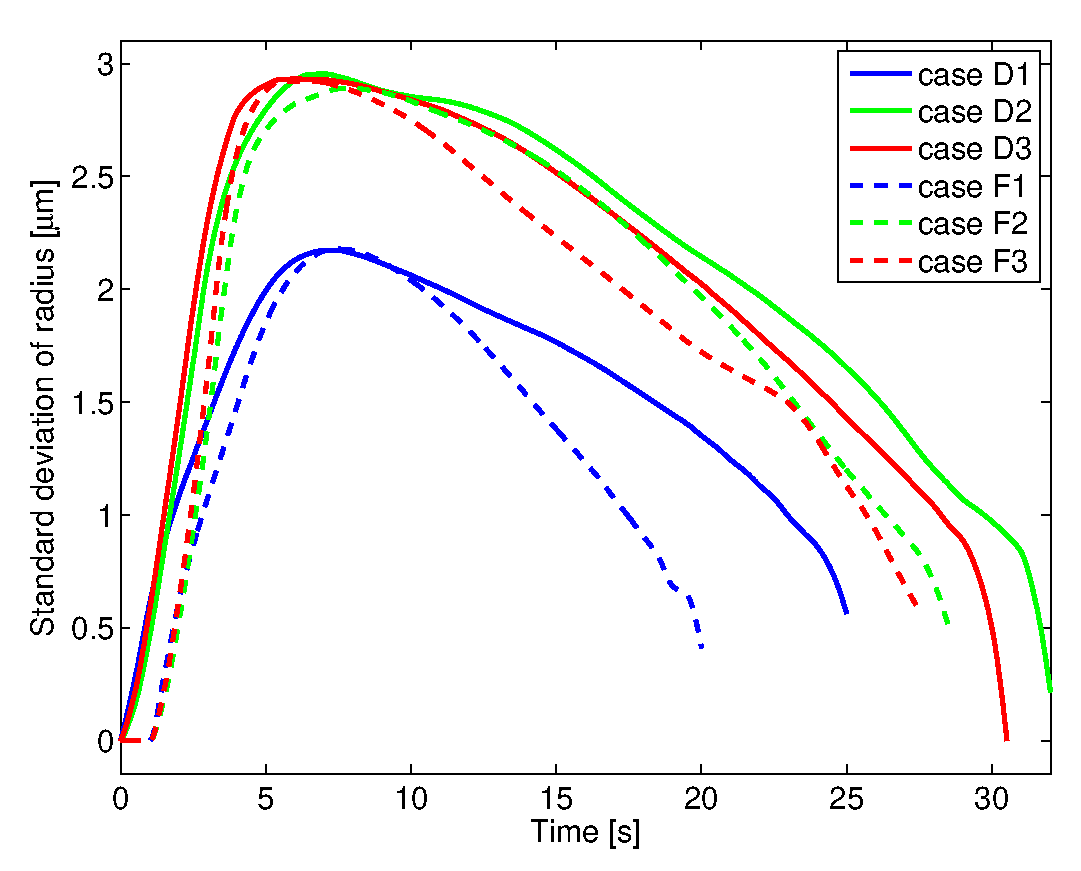
\includegraphics[width=0.48\linewidth]{Figures/std_radius}
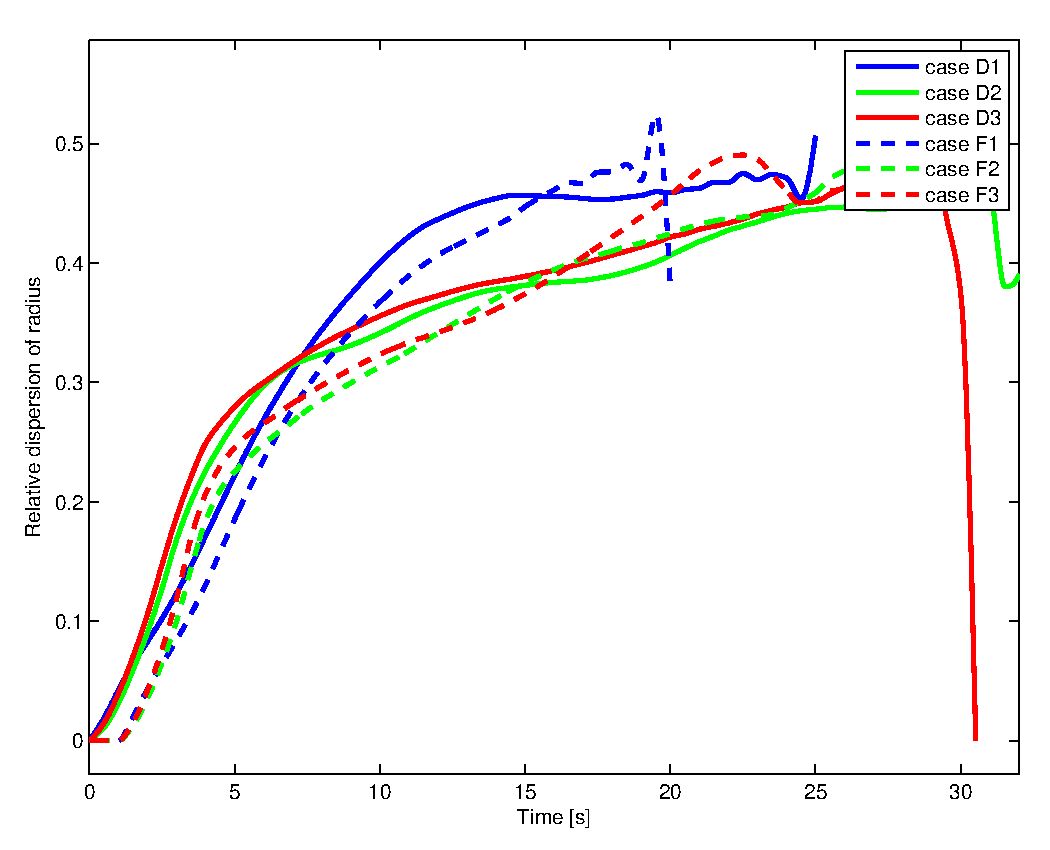
\includegraphics[width=0.48\linewidth]{Figures/dsp_radius}
\caption{From top to bottom and left to right are temporal evolutions of (a) droplets concentration, (b) liquid water content, (c) mean volume radius, (d) mean radius, (e) standard deviation and (f) relative dispersion.}\label{fig:temporal_variation} 
\end{figure}

Note that a droplet with radius smaller than $1\mu m$ will be immediately removed from the computational domain, and therefore will not contribute to any statistical results.

In summary, the shape of the cloud filament has no influence on the final state after the mixing but will affect the intermediate process, but cannot be completely ignored for their intermediate states. The results suggest that the initial shape of cloud filaments should be considered as an important factor when studying mixing scenario with or without external forcing. All cases have the same equilibrium state with a zero liquid water content, i.e. all droplets eventually evaporate. The rate at which droplets evaporate is higher for the forced turbulence than the decaying turbulence except D1, in which all the droplets are quickly exposed to the same environment and begin to evaporate, leading to its number concentration curve to be similar as the forced case.

\section{Turbulent entrainment-mixing processes}\label{mixing_processes}

\subsection{Mixing diagram analysis}
Turbulent entrainment of dry environmental air and subsequent turbulent mixing between cloudy air and environmental air and associated droplet evaporation are likely primary factors that affect the droplet size distributions and corresponding microphysical properties. There are two limiting entrainment-mixing mechanisms proposed in the literature. One is that the entrained air and the cloudy air are mixed evenly and all cloud droplets evaporate with the same proportion \cite{Warner1973}. This type of mixing is referred to as homogeneous mixing. The other type of mixing is inhomogeneous mixing, where the entrained air mixes with only some portion of cloud parcel and evaporate all droplets in this portion completely while the droplets in the rest of the cloud parcel remain intact \cite{Baker1980}. Ambient clouds often fall between the two limiting mechanisms. To characterize the effect of turbulent entrainment-mixing processes on microphysical properties, the $R_v^3-N_c$ diagram was introduced in \cite{Burnet2007Observational}, and has been widely applied to study the homogeneous/inhomogeneous entrainment-mixing process in observational studies and DNS simulations. \cite{And04, And06, And09} were probably the first studies that applied the mixing diagram analysis to DNS simulations with bin microphysics. \cite{Kumar14} further applied to the mixing diagram analysis to their particle-resolved DNS simulations. In addition to their model differences,  \cite{And04, And06, And09} used Case 1 initial configuration of cloudy area whereas Kumar et al used a configuration similar to our Case 2. This section extends these pioneering studies to examine the results of all the six scenarios by use of the mixing diagram analysis.

In addition to the domain mean as examined by Andrejczuk et al, we also examine smaller averaging boxes to obtain better ideas of statistics by following Kumar et al. \cite{Kumar14} to divide the computational domain into 64 equal-sized sample boxes. We keep tracking the volume mean radius and number concentration at each time step in each sample box. \Fig{fig:mixing_diagram} shows the mixing diagrams for the six scenarios. The solid green dot represents the value sampled in each sample box at each time step; the red curve denotes the DNS domain average, with arrows indicating the direction of temporal evolution. The corresponding homogeneous mixing line (black dot) and extreme inhomogeneous mixing line (black solid) are plotted in the diagram as references. Note that in the top panel, the mixing diagrams for D1 and F1 do not start from the $(1,1)$ point since the initial droplets in a sample box have already been diluted and their number concentration are thus less than the adiabatic value. The droplet number concentration remains nearly unchanged as the droplet size decreases until some time has elapsed, suggesting an extreme homogeneous mixing.  The difference between forced turbulence and decaying turbulence is not obvious, except a wider range of variability in the shape of the mixing trajectories for the decaying turbulence D1, since the forced turbulence will foster the mixing procedure, resulting in similar states in different sample boxes. As claimed in \cite{And04}, this configuration excludes the initial dilution process and can only be used to simulate the mixing process after dilution.

The middle panel shows the mixing diagrams for case D2 and F2. These cases have the same configurations with \cite{Kumar14}. However, a sharp initial profile of vapor mixing ratio was used in our simulation. This results in an unsaturated vapor mixing ratio at final state, leading to completely evaporation of the droplets. The phenomenon of inhomogeneous offset described by \cite{Kumar14} can also be observed in the figures: the mixing trajectories tend to shift to smaller values of $N_c/N_{c,a}$. This inhomogeneous offset is due to the initial dilution process, in which the droplets number concentration in the sample boxes is diluted while the droplets mean radius in the sample box doesn't change too much. As mixing proceeds, the turbulent time scale in the decaying case continues to increase while the time scale for the forced turbulence remains unchanged. Therefore, the inhomogeneous mixing is more likely to occur in D2, leading to a slightly stronger deviation from the homogeneous mixing line.  A similar conclusion can be obtained in the bottom panel for case D3 and F3. 

It is noteworthy to observe that the points in Case 3 are more scattered than other cases in the mixing diagrams. During the initial several seconds, a part of the points move along the inhomogeneous line and others are below the red curve and closer to the homogeneous line. As mixing proceeds, this two groups move towards $(0,0)$ point and finally merge together. We interpret this divergence by considering the following facts. According to our way of selecting sample boxes, the cloud slab will be divided into two groups: the upper layer and the lower layer. On one hand, due to the sedimentation effect, a part of the droplets will escape from the upper layer and enter into the lower layer, thus making the number concentration of upper level sample boxes decreased and their volume mean radius unchanged. On the other hand, the evaporating droplets below the lower layer may reentering into the lower sample boxes by the turbulent mixing, leading to reduced volume mean radius and slowly decreasing number concentration. 

Also noteworthy is that the difference between the mixing diagrams lies primarily in the cloudy area configurations, esp., Case 1 vs. Case 2 or Case 3, instead of lying in whether or not the turbulence is forced or freely decaying as shown \Fig{fig:rad_distri} and \Fig{fig:supersat_distri} for the temporal evolutions of droplet size distribution and supersaturation, respectively.  This result suggests the potential for a unifying parameterization of different mixing mechanisms detailed next.

\begin{figure}[!htbp]\centering
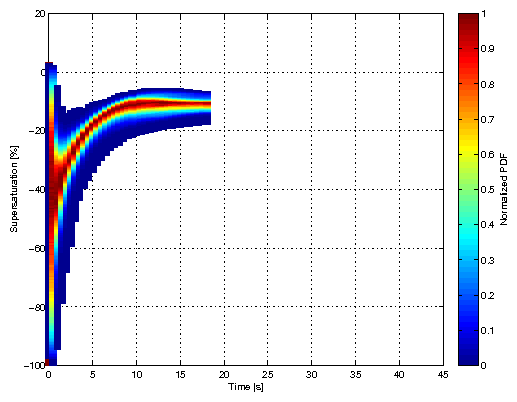
\includegraphics[width=0.48\linewidth]{Figures/pdf_supersat_d1}
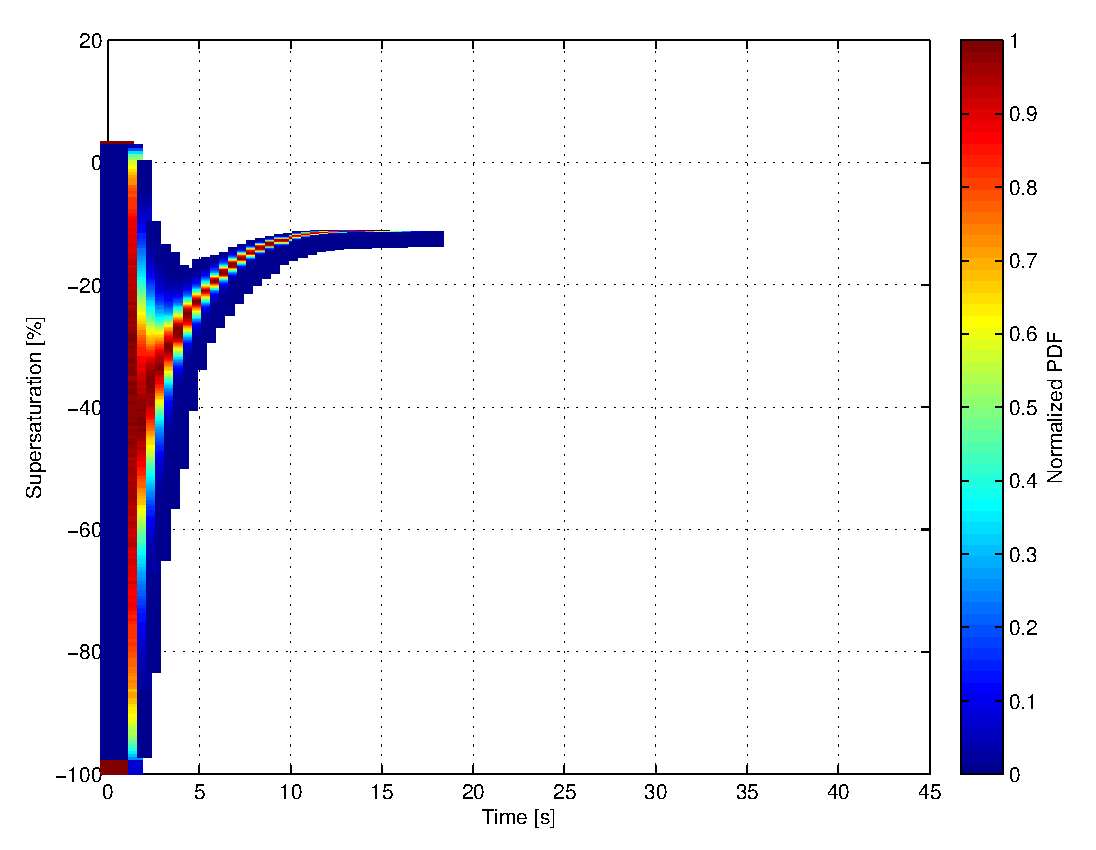
\includegraphics[width=0.48\linewidth]{Figures/pdf_supersat_f1}\\
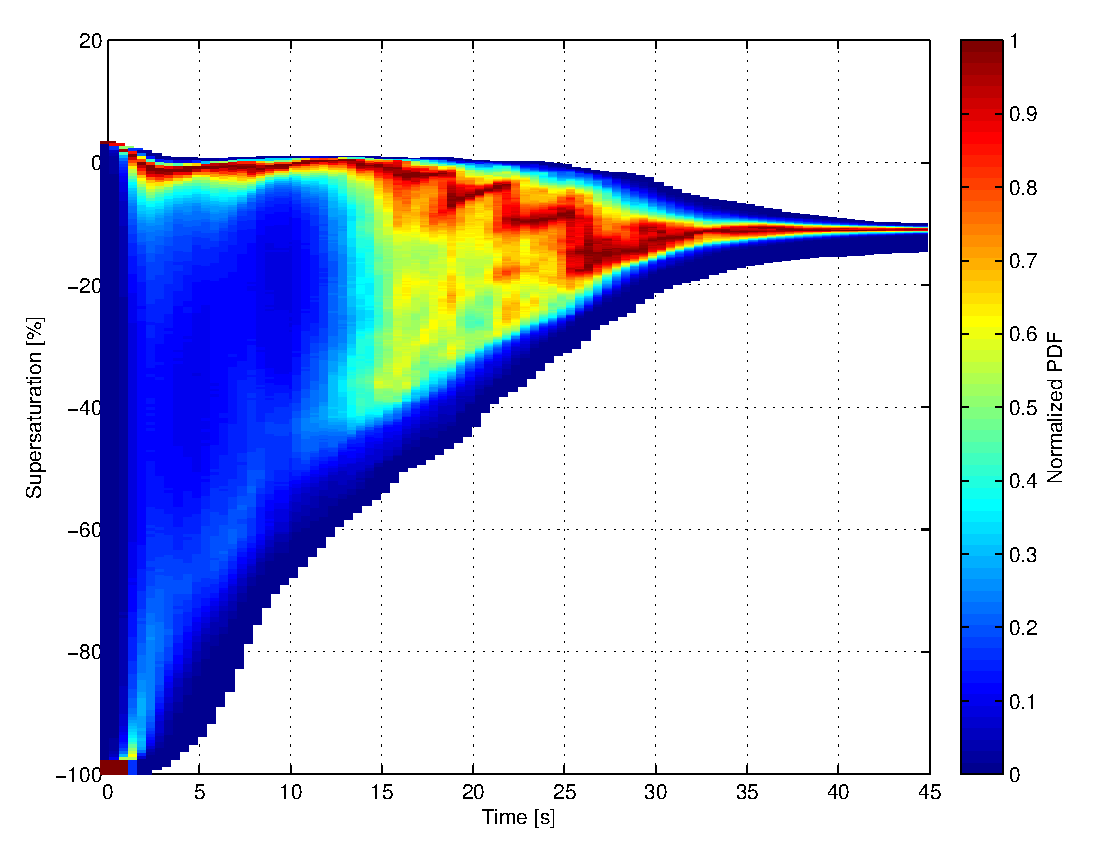
\includegraphics[width=0.48\linewidth]{Figures/pdf_supersat_d2}
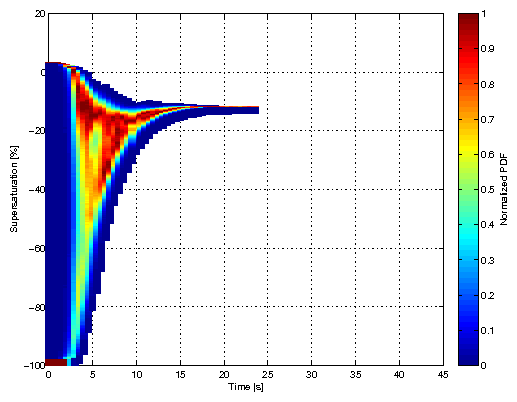
\includegraphics[width=0.48\linewidth]{Figures/pdf_supersat_f2}\\
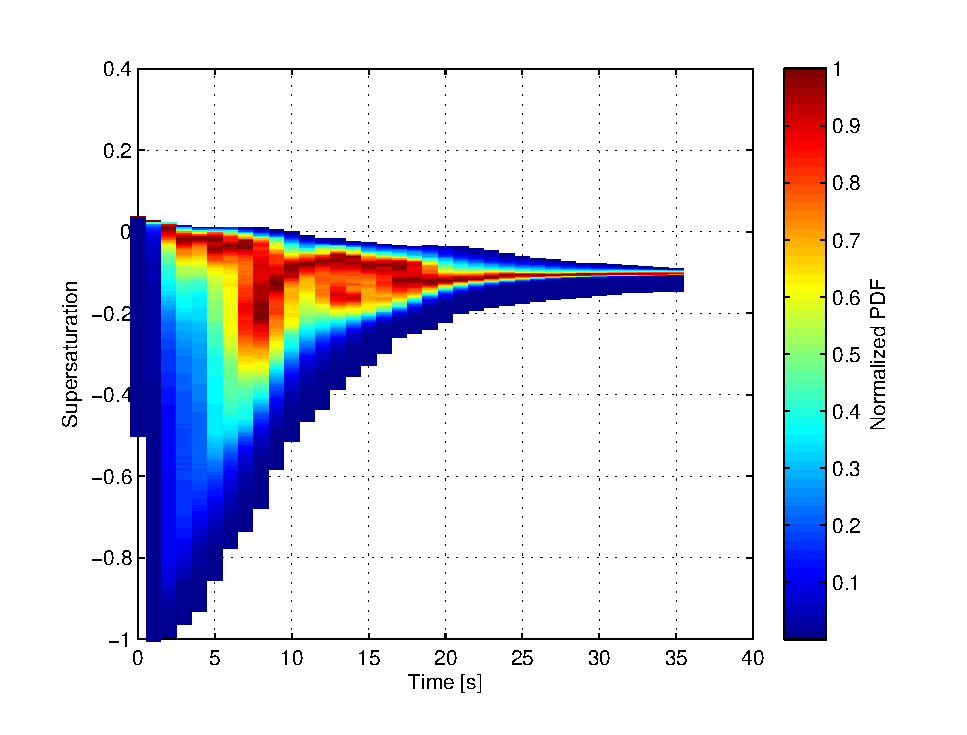
\includegraphics[width=0.48\linewidth]{Figures/pdf_supersat_d3}
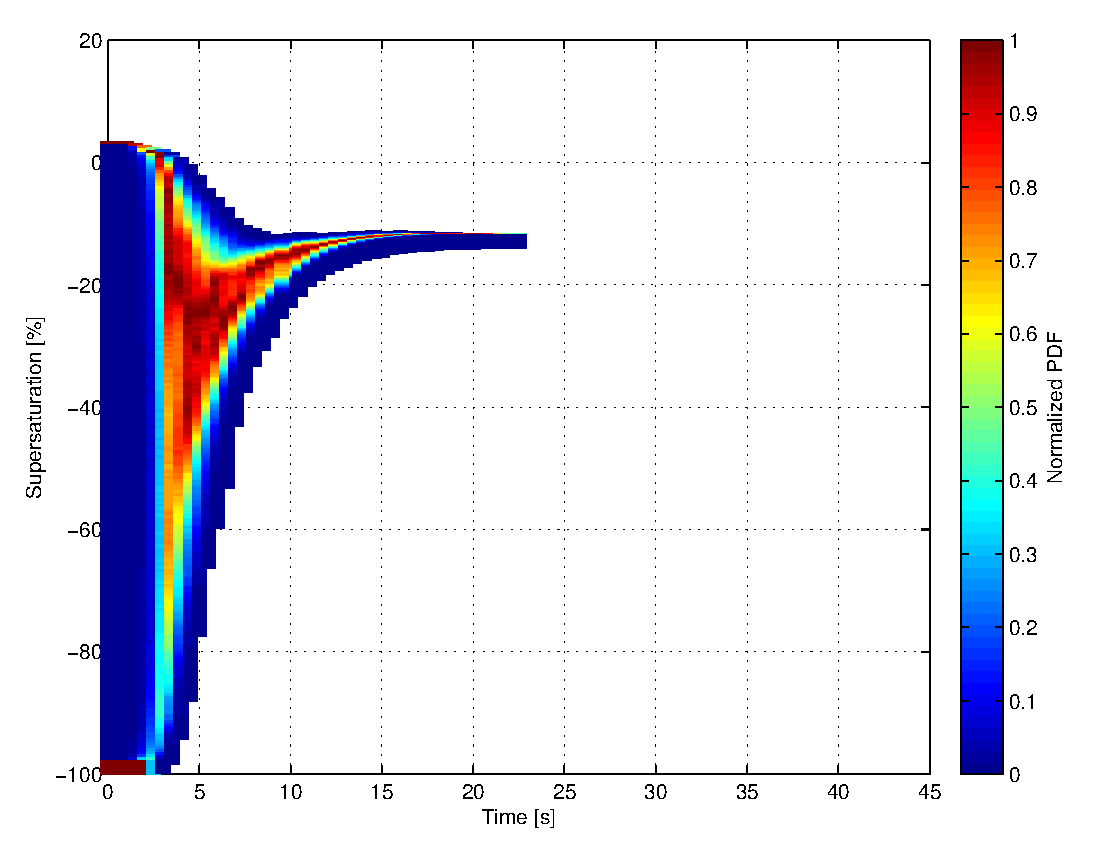
\includegraphics[width=0.48\linewidth]{Figures/pdf_supersat_f3}
\caption{Evolution of supersaturation distribution for decaying turbulence (left column) 
and forced turbulence (right column). From up to bottom are case 1, case 2 and case 3 respectively.}\label{fig:supersat_distri}
\end{figure}

\begin{figure}[!htbp]\centering
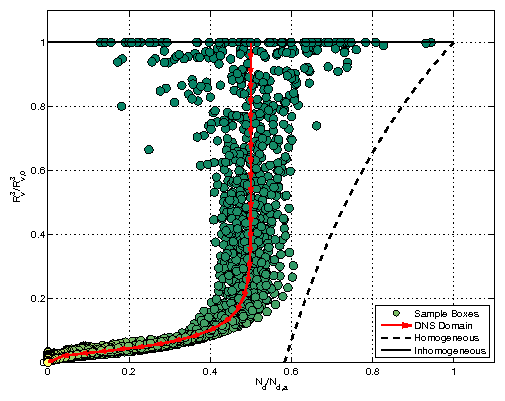
\includegraphics[width=0.4\linewidth]{Figures/mixing_cased1}
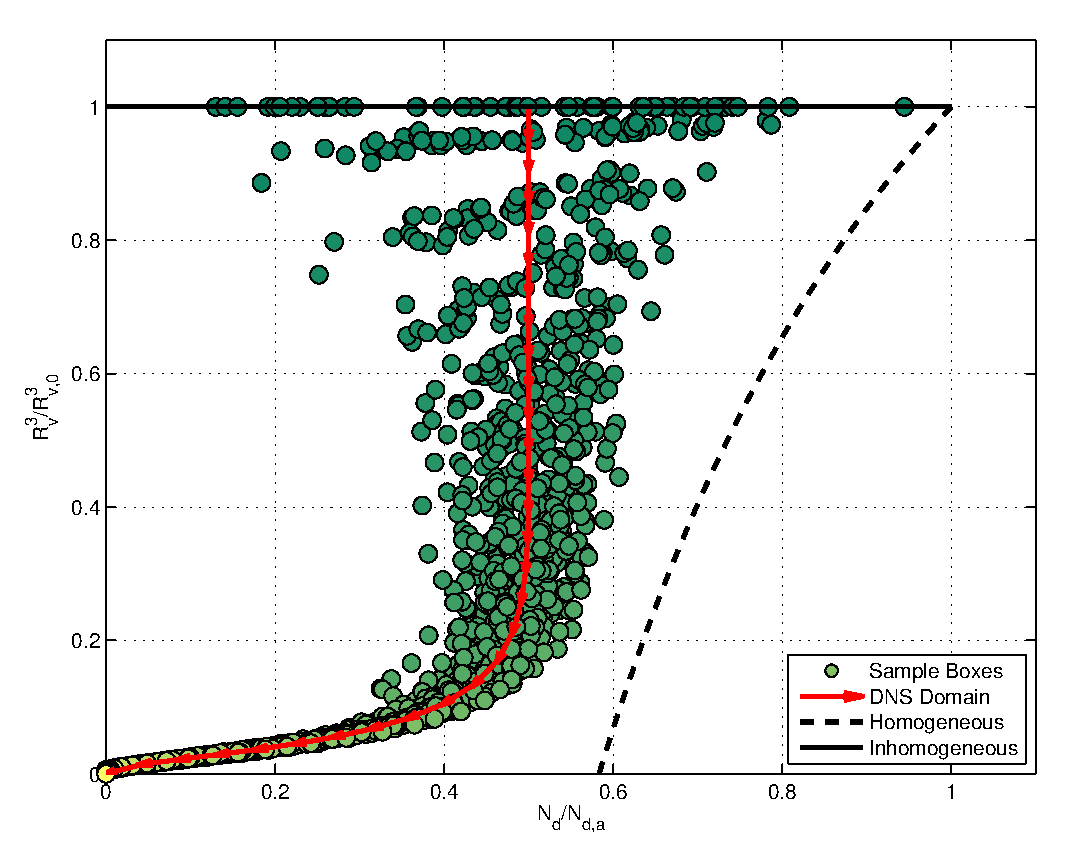
\includegraphics[width=0.4\linewidth]{Figures/mixing_casef1}
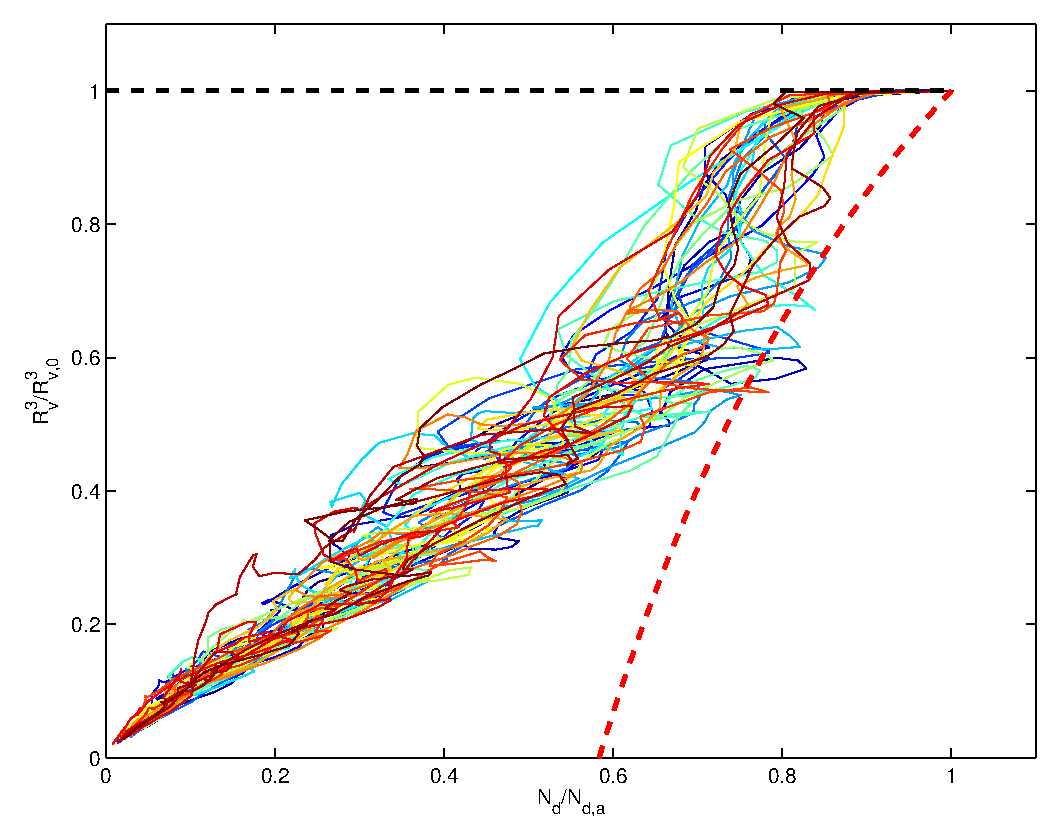
\includegraphics[width=0.4\linewidth]{Figures/mixing_cased2}
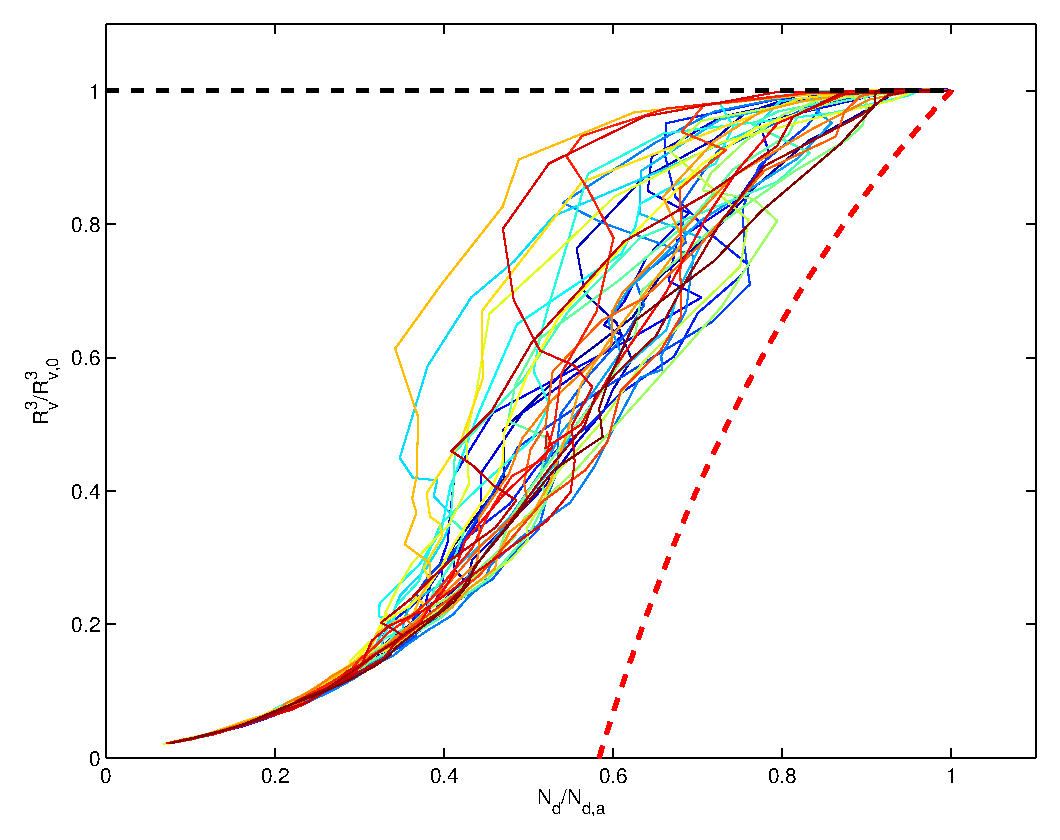
\includegraphics[width=0.4\linewidth]{Figures/mixing_casef2}
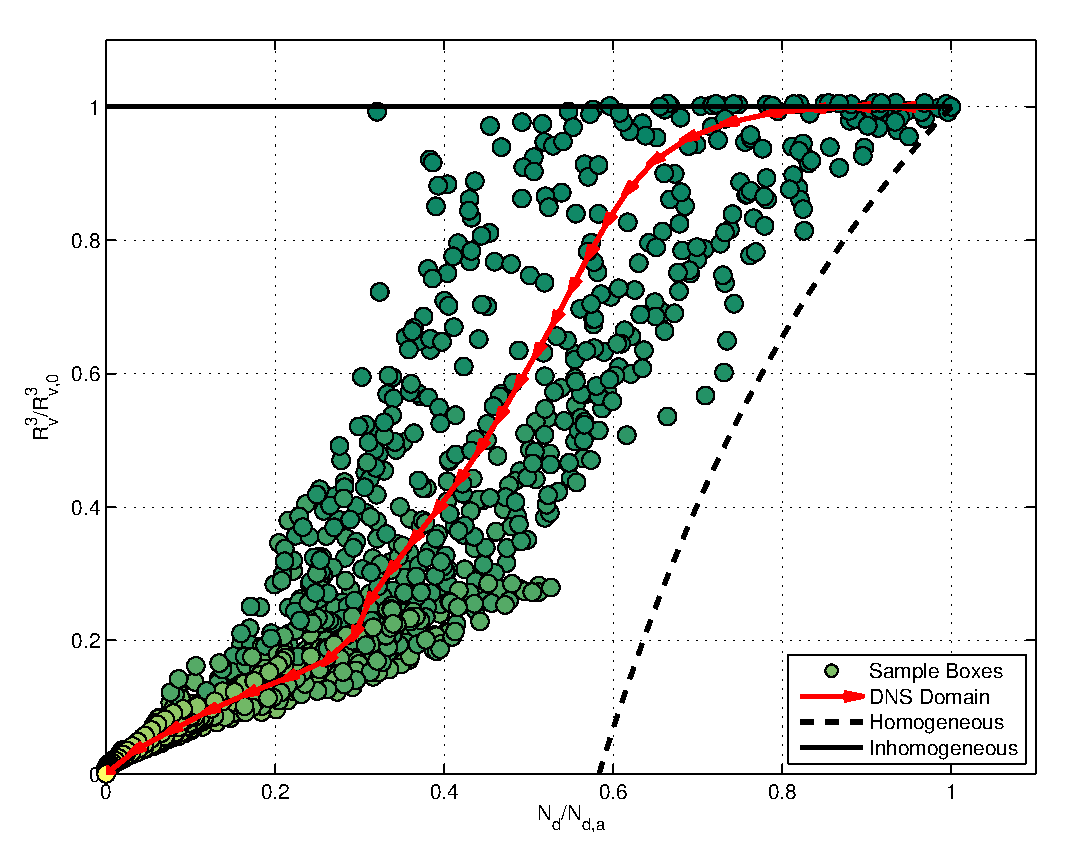
\includegraphics[width=0.4\linewidth]{Figures/mixing_cased3}
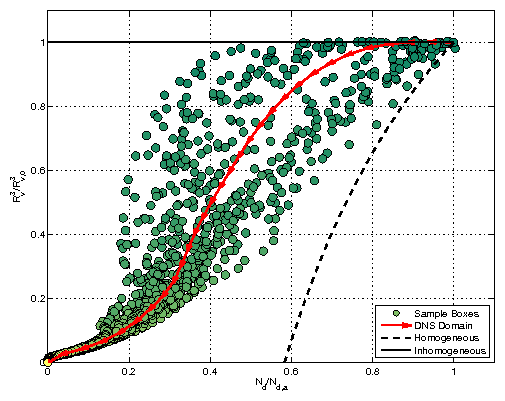
\includegraphics[width=0.4\linewidth]{Figures/mixing_casef3}
\caption{Mixing diagram for case D1, D2, D3, F1, F2 and F3. Mean cubic radius
and mixing fraction have been calculated in 64 equal-sized samples boxes. The
circle represent the time trajectories of $R_v^3/R_{v,0}^3$ and $N_d/N_{d,a}$
in different sample boxes and the triangles represent the same in the entire
domain. Color indicates the time for each record. Only the boxes with non-zero
particles at the initial time are considered.}
\label{fig:mixing_diagram}
\end{figure}

\subsection{Microphysical measures for different mixing mechanisms}
Since the real entrainment-mixing mechanism can fall anywhere between the limiting mixing mechanisms, it is desirable to define some measure that covers all the possible mixing processes. We generically called such a measure as homogeneous mixing degree since a larger homogeneous mixing degree indicates that the mixing process is closer to the limiting homogeneous mixing process. Based on the fact that the horizontal line in the $R^3−N_c$ diagram corresponds to the extremely inhomogeneous mixing whereas the vertical line implies extremely homogeneous mixing \citep{And09}, the homogeneous mixing degree can be quantified by the instantaneous slope of the trajectories in the mixing diagram, and is calculated using central differencing in time: 
\begin{equation}
\psi_1 = \frac{R_{j+1}^3/R_a^3 - R_{j-1}^3/R_a^3}{N_{j+1}/N_a - N_{j-1}/N_a}
\label{phi0}
\end{equation}
where the subscript ``$a$'' denotes the adiabatic value of the droplet population in the initial cloudy region. Note that $\psi_1$ is in fact the inverse of the slope defined by \citep{And09} such that a larger value of $\psi_1$ indicates a higher degree of homogeneous mixing, in line better with intuition and the other microphysical measures discussed below.

More measures of homogeneous mixing degree have been introduced in \cite{Lu2011, Lu2014}. 
These measures are based on the mixing of adiabatic cloudy air and clear air, and slightly 
modified here to consider the instantaneous homogeneous mixing degree between two adjacent 
temporal states in time $t_j$ and $t_{j-1}$, such that
  
\begin{equation}
\psi_2 = \frac{\tan^{-1}(\frac{R_{j}^3/R_{j-1}^3 - 1}{N_j/N_{j-1} - N_H/N_{j-1}})}{\pi/2}
\label{phi1}
\end{equation}

\begin{equation}
\psi_3 = 0.5(\frac{N_j-N_{I}}{N_H-N_I} + \frac{R_j^3-R_{j-1}^3}{R_H^3 - R_{j-1}^3})
\label{phi2}
\end{equation}

\begin{equation}
\psi_4 = \frac{\ln R_j^3 - \ln R_{j-1}^3}{\ln R_{H}^3 - \ln R_{j-1}^3}
\label{phi3}
\end{equation}

\begin{equation}
\psi_5 = \frac{1 - R_{j}^3/R_{j-1}^3}{1 - LWC_{j}N_{j-1}/(N_H LWC_{j-1})}
\label{phi4}
\end{equation}

where all the variables are calculated from a sample box; $R$ is the mean volume radius; $N$ is the number concentration; $LWC$ is the liquid water content; the subscript ``$j$'' means the value is calculated from the $j$-th dataset at time $t_j$. The subscripts $I$ and $H$ indicate that the values are calculated based on the assumption of inhomogeneous and homogeneous mixing, respectively. Briefly,
\[
N_H = \chi N_j + (1 - \chi) Ne_j
\]

\[
R_H^3 = \frac{N_jR_j^3}{N_H},
\]

\[
N_I = \frac{R_j^3}{R_{j-1}^3}N_j.
\]



The mixing fraction $\chi$ is computed according to the mass conservation of total water between state $j$ and $j-1$:
\begin{equation}
\chi(q^{j-1}_{vc} + q^{j-1}_{lc}) + (1-\chi)(q^{j-1}_{ve} + q^{j-1}_{le}) = q^{j}_{lc} + q^{j}_{vc}
\label{eq:mixing_frac}
\end{equation}
where the subscripts $c$ and $e$ stand for the mean 
value of a sample box and its environmental air; $l$ and $v$ stand for the liquid 
water and water vapor. The environmental air is defined as the air in $4$ 
grids extended from the original sample box; the subscript $j$ indicates the state of the $j$-th dataset 
collected at time $t_j$. Note that \Eq{eq:mixing_frac} considers the fact that the cloudy air may have 
been diluted and the environmental air may contain droplets.

It can be readily shown that $\psi_1$ equals to $0$ for the extremely inhomogeneous mixing, but 
approach $\infty$ as the mixing process approaches homogeneous mixing. On the other hand, the 
other four definitions of homogeneous mixing degree all range between $0$ and $1$, with $0$ for 
extremely inhomogeneous mixing and $1$ for homogeneous mixing. 
Note that the theoretic range of $\psi_1$ is $[0, \infty]$ while $\psi_2$, $\psi_3$, $\psi_4$ and $\psi_5$ 
are $[0, 1]$, and therefore it is difficult to compare $\psi_1$ with other measures.
\Fig{phi_compare} compares the four measures of homogeneous mixing degree whereby each dot represents an 
instantaneous domain-mean and the different color denotes the six different scenarios.
As expected, all the measures of homogeneous mixing degree are positively related 
to one another, and can be used as a microphysical measure to quantify the entrainment-mixing process.
\begin{figure*}[!htbp]\centering
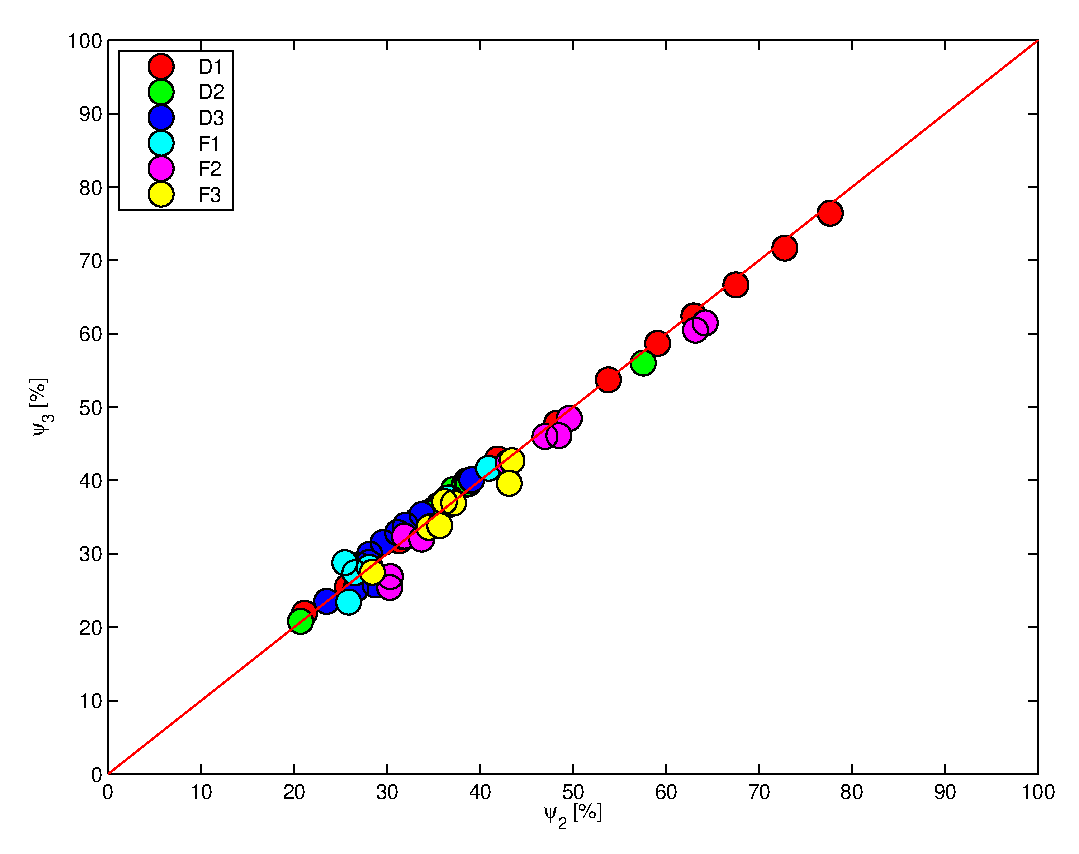
\includegraphics[width=0.3\linewidth]{Figures/phi2_phi3}
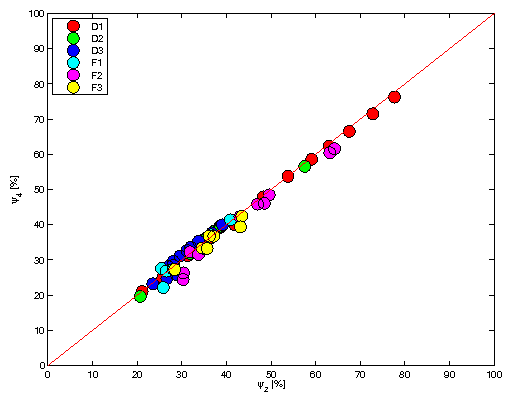
\includegraphics[width=0.3\linewidth]{Figures/phi2_phi4}
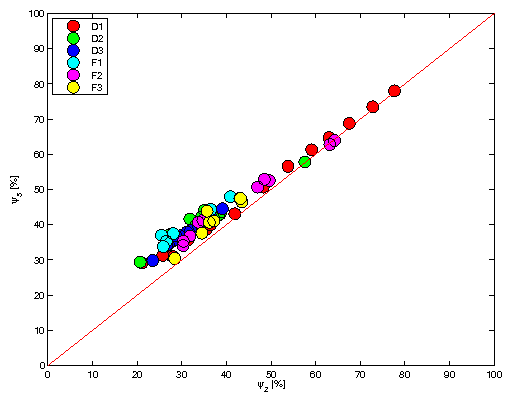
\includegraphics[width=0.3\linewidth]{Figures/phi2_phi5}
\caption{Comparison between different mixing degree, from left to right are $\psi_2$ with $\psi_3$, $\psi_4$ and $\psi_5$.\label{phi_compare}}
\end{figure*}

\subsection{Analysis of dynamical measures}
Following the previous work contributed by 
\cite{Krueger1997Modeling,Grabowski1993Cumulus, Burnet2007Observational}, 
the entrainment-mixing process can be characterized by the Damk{\"o}hler number, the ratio of 
turbulent mixing timescale to a microphysical timescale:

\begin{equation}
Da=\frac{\tau_{mix}}{\tau_{react}}\label{eq:DaNumber}
\end{equation}
where the turbulence mixing time scale can be estimated as $\tau_{mix} = (\lambda^2/\epsilon)^{1/3}$; the length scale $\lambda$ is represented by the mean Taylor microscale for the cloud water, $\lambda = 
(\lambda_1+\lambda_2+\lambda_3)/3$, $\lambda_i = \langle q_c^2\rangle^{1/2}/\langle(\partial q_c/\partial x_i)^2\rangle^{1/2}$, and the dissipation rate is estimated with $\epsilon = 2\nu\langle(\nabla\times \mathbf{u})^2\rangle$. The definition of reaction time scale $\tau_{react}$ will be introduced later. In general, $Da\ll1$ corresponds to the homogeneous mixing while $Da\gg1$ is
the inhomogeneous one. Ambient clouds often have $Da$ between these two limits.

Recognizing that the turbulent mixing time scale depends on the entrained eddy sizes, 
\cite{Lehmann2009} introduced the transition length scale defined as the length scale at 
which $Da = 1$. A larger transition scale length suggests a higher degree of homogeneous mixing. 
It can be shown
\[
l^{*}=\epsilon^{1/2}\tau_{react}^{3/2}
\]

\cite{Lu2011} further introduced the transition scale number defined as the ratio of 
transition length to Kolmogorov length scale as a dynamic measure of homogeneous mixing degree:
\begin{equation}
N_{L}=\frac{l^{*}}{\eta}\label{eq:NL}
\end{equation}
where the Kolmogorov length scale is given by
\[
\eta = (\frac{\nu^3}{\epsilon})^{1/3}, 
\]


In \cite{Lehmann2009, Lu2013}, $\tau_{react}$ is defined as the time when droplets have completely 
evaporated or relatively humidity has reached $99.5\%$ whichever is first satisfied. It is calculated 
by solving the following ordinary differential equation for the mean volume radius and mean supersaturation:
\begin{equation}
\frac{dR_{v}}{dt}=K\frac{S}{R_{v}}\label{eq:DiffR}
\end{equation}

\begin{equation}
\frac{dS}{dt}=-BR_{v}S\label{eq:DiffSuper}
\end{equation}
where $B$ is a function of pressure and temperature:
\begin{equation}
B = 
\frac{4\pi N\rho_L[\frac{G_dT}{\varepsilon e_s(T)} + \frac{\varepsilon L^2_h}{pTc_p}]} 
{(\frac{L_h}{G_vT}-1)\frac{L_h\rho_L}{\mu_T T} + \frac{\rho_L G_v T}{\mu_v e_s(T)}}
\end{equation}

where $L_h$ is latent heat, $G_v$ is individual gas constant for water vapor,
$T$ is air temperature, $\rho_L$ is density of liquid water, $\mu_T$ is coefficient
of thermal conductivity of air, $\mu_v$ is coefficient of diffusion of water vapor
in air, $e_s(T)$ is saturation vapor pressure over a plane water surface at
temperature $T$, $N$ is number concentration of droplets, $G_d$ is individual
gas constant for dry air, $\varepsilon = G_d/G_v$, $p$ is air pressure, and
$c_p$ is specific heat with pressure held constant (\cite{Lu2011}).
This definition considers the interactions between liquid water and vapor water, 
and hence its value is expected to be smaller than the previous definition. 

Another microphysical time scale is the so-called evaporation time defined as the time that a droplet needs to complete the evaporation \cite{Andrejczuk2009, Burnet2007Observational}:
\begin{equation}
\tau_{evap} = R_v(\frac{dR_v}{dt})^{-1} = \frac{R_v^2}{-KS_e}
\end{equation}
where $R_v$ is the mean volume radius of a group of droplets; $K$ is the constant in the 
droplet diffusional growth equation, and $S_e$ is the supersaturation of the dry air.
Evidently, the evaporation time scale assumes that the environmental dry air is always 
unsaturated with a constant negative $S_e$.
 
\subsection{Parameterization of entrainment-mixing processes}
The impact of entrainment and cloudy-clear air mixing on the spectra of cloud droplets remains an important yet still unresolved issue in cloud physics. Because warm (ice free)
clouds are close to water saturation, conservation of the total water and moist static energy is sufficient to determine the temperature, water vapor, and cloud water mixing ratios of the homogenized mixture of cloudy and cloud-free unsaturated air. Predicting the evolution of a cloud droplet spectrum, on the other hand, requires additional constraints because, as far as bulk conservation principles are concerned, cloud water after homogenization can be distributed over either a large number of small droplets or a small number of large droplets. The concentration and size of cloud droplets critically depend on whether the mixing is homogeneous (i.e., all droplets are exposed to the same subsaturation during mixing) or inhomogeneous (i.e., the degree of droplet evaporation varies; \cite{Baker1979, Baker1980, Burnet2007Observational}. In the homogeneous mixing scenario, the number of droplets does not change and the mean droplet size decreases. In the extreme inhomogeneous mixing scenario, droplets from a fraction of the cloudy volume evaporate completely to bring the mixture to saturation, and the droplets from the rest of the cloudy volume are dispersed over the combined volumes without
changing their size. It follows that the extremely inhomogeneous mixing is associated with the change of droplet concentration, but not the droplet size. The homogeneous mixing and the extremely inhomogeneous mixing set the limits for all possible mixing scenarios. Whether cloud dilution is associated with homogeneous or inhomogeneousmixing has been shown to significantly affect radiative properties of stratocumulus \cite{Chosson2007} and shallow convective clouds \cite{Grabowski2006, Slawinska2008}.

\cite{Burnet2007Observational} showed that the Damk\"{o}hler number, defined as the ratio between the mixing time scale ($\tau_m$) of dry air and cloud air and the evaporation time scale ($\tau_e$) could be used as a parameter that indicates which mixing mechanism is dominant. \cite{Lehmann2009} argued that the mixing mechanism could be better determined with the transition length scale instead of the Damk\"{o}hler number because of the uncertainty in knowing the turbulent mixing length scale. The results varied by cloud region; homogeneous mixing (HM) appeared more frequently in the vicinity of the cloud core, while inhomogeneous mixing (IM) appeared more frequently in more diluted cloud regions \cite{Lehmann2009}. Similarly, \cite{Lu2011} proposed that the transition scale number defined as the ratio of transition length to the Kolmogorov length scale could be used as a parameter to estimate mixing mechanisms; a higher transition scale number corresponds to a greater tendency of homogeneous mixing.
The transition scale number \Eq{eq:NL}, Damk\"{o}hler number \Eq{eq:DaNumber} and the various microphysical measures of homogeneous mixing degree \Eq{phi0}, \Eq{phi1}, \Eq{phi2}, \Eq{phi3} and \Eq{phi4} are expected to be correlated since they are two measures quantifying the probability of the homogeneous mixing process from different perspective. These relationships are examined using the numerical data produced from the six simulations.  First, the slope \Eq{phi0} is plotted against the Damk\"{o}hler number and transition scale number in \Fig{fig:slope_da_nl}. The left figure shows that the Damk\"{o}hler number has a positive relationship with the reciprocal of the slope. This duplicates the results in \cite{And09} and is consistent with the heuristic argument relating homogeneity of mixing to the time scale ratio. We also compare the results using transition scale number and Damk\"{o}hler number as the dynamical measures in the right figure. It yields that the transition scale number has a wider range of values but gives consistent conclusion with Damk\"{o}ler number.

\begin{figure}[!htbp]\centering
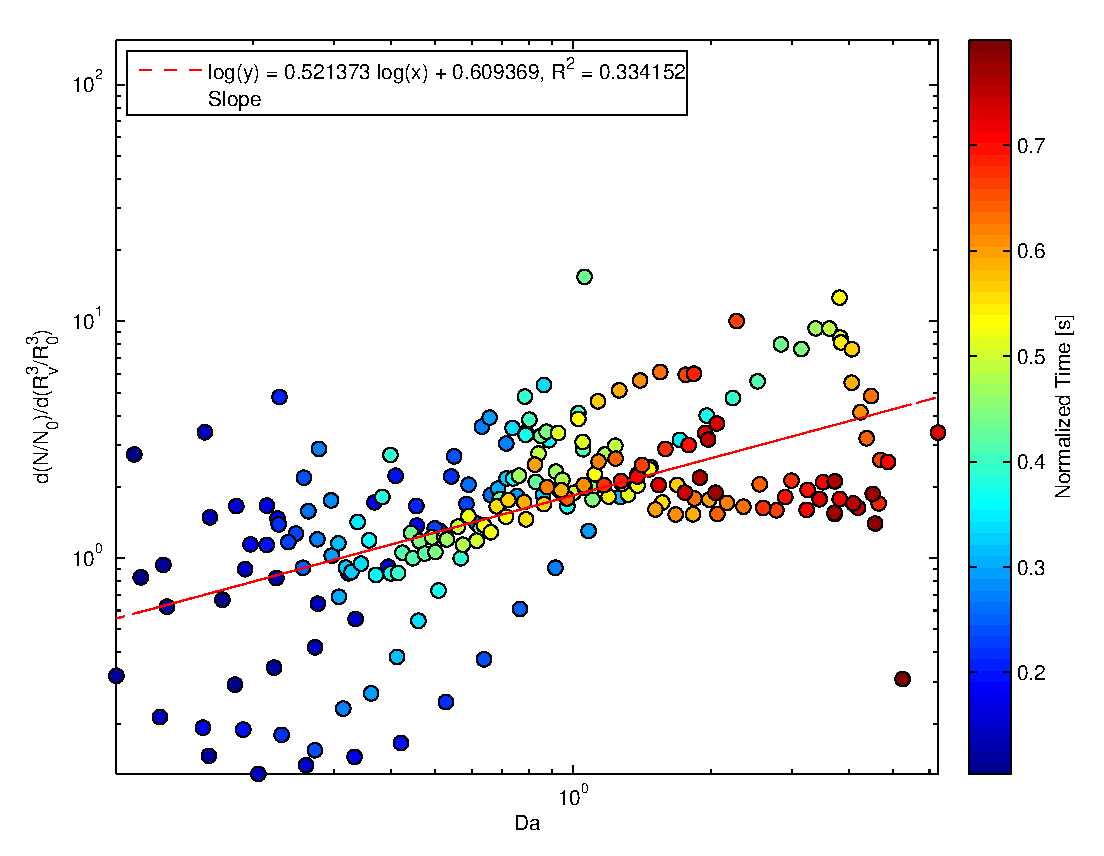
\includegraphics[width=0.49\linewidth]{Figures/slope_da}
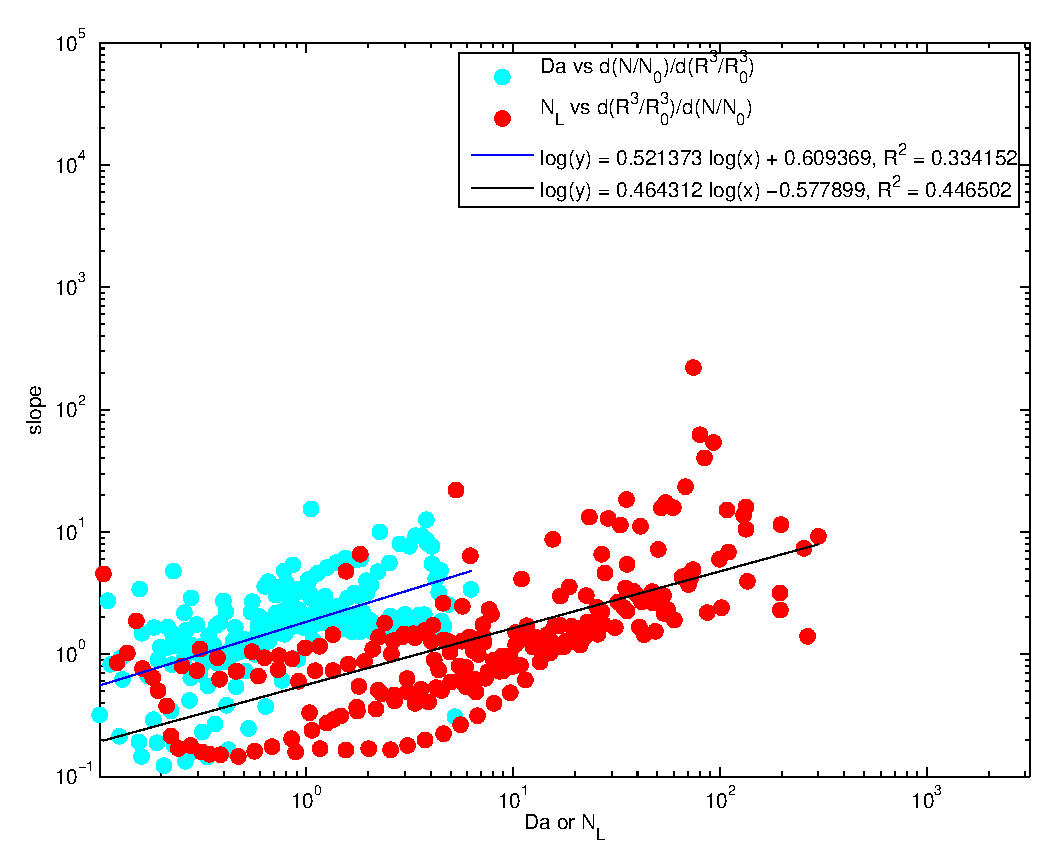
\includegraphics[width=0.49\linewidth]{Figures/slope_da_nl}
\caption{The left figure displays the scatter plot of the slope in the $R-N$ diagram as a function 
of Damk\"{o}hler number and transition scale number. The comparison between using Damk\"{o}hler 
number and transition scale number is shown in the right figure.}
\label{fig:slope_da_nl}
\end{figure}

The scatterplot of the homogeneous mixing degree as a function of the transition scale number is shown in \Fig{fig:mix_degree_nl} with color indicating the normalized simulation time. The fitting curves have a close slope for different cases, and a tight relationship can be observed in the critical range of the slopes, and therefore one can suggest a simple parameterization.
\begin{figure}[!htbp]\centering
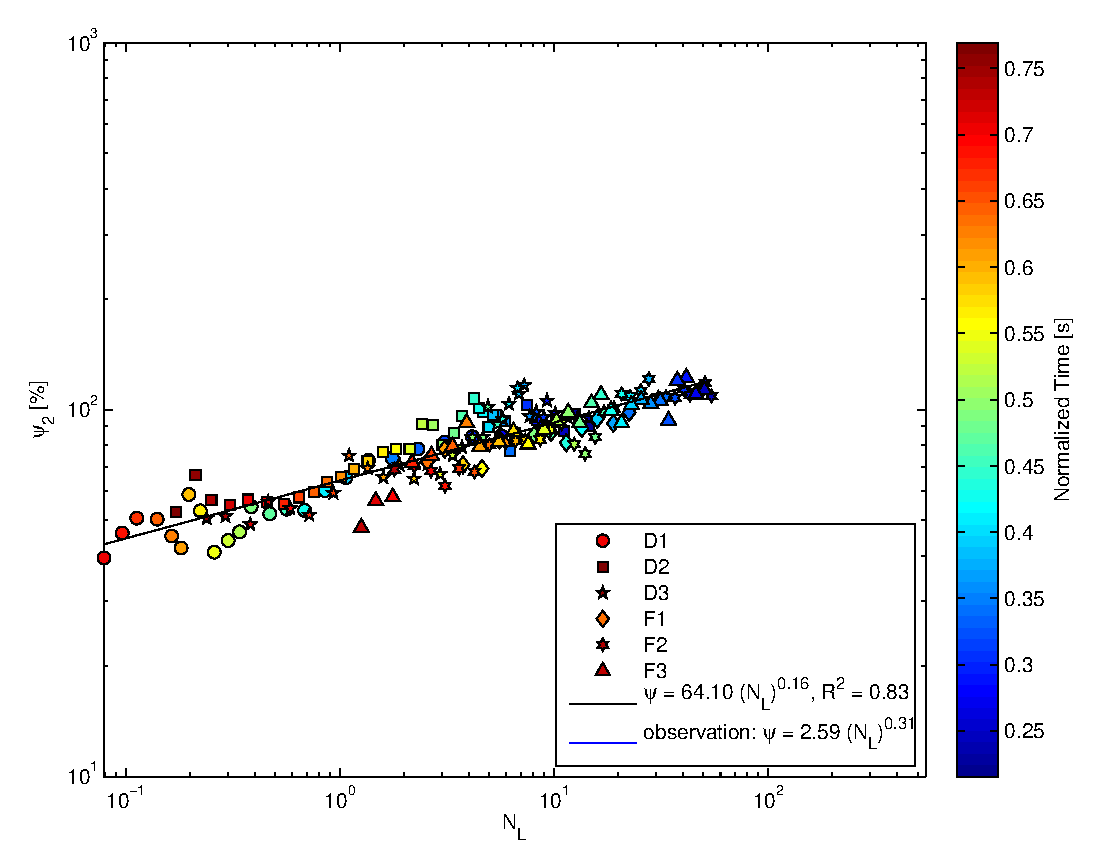
\includegraphics[width=0.49\linewidth]{Figures/phi2nl}
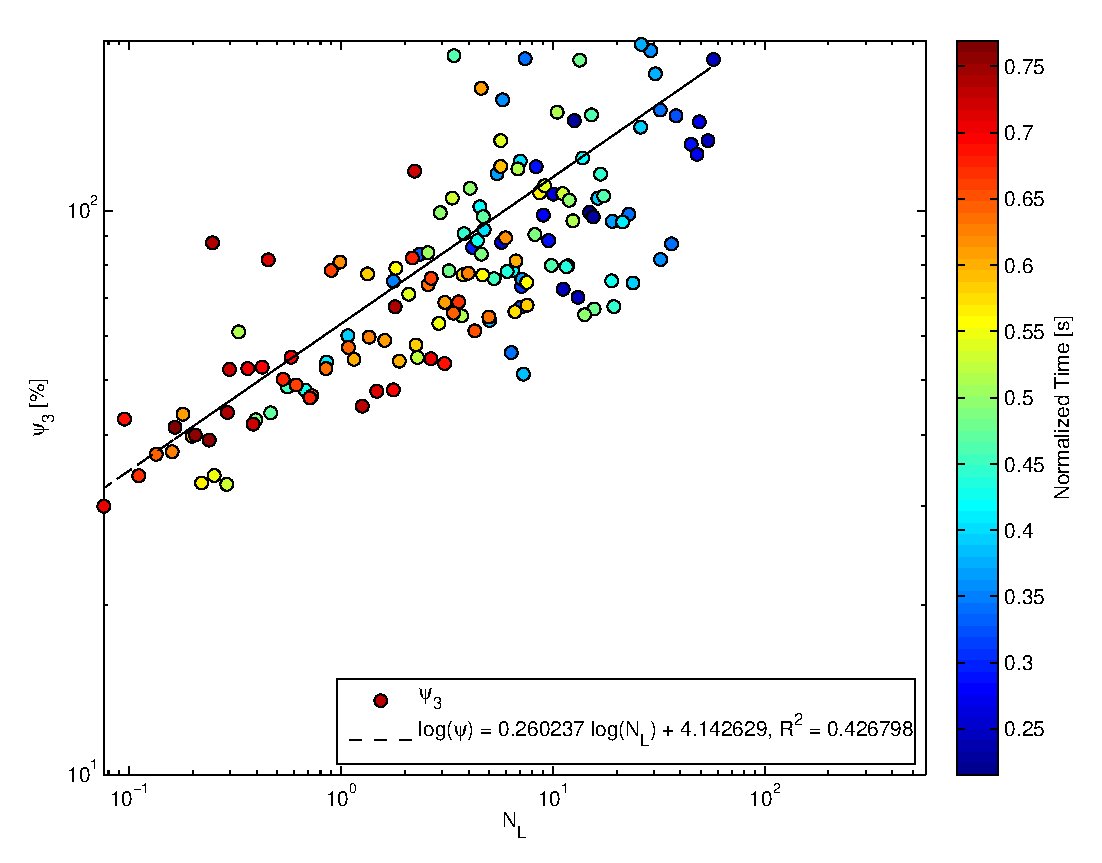
\includegraphics[width=0.49\linewidth]{Figures/phi3nl}\\
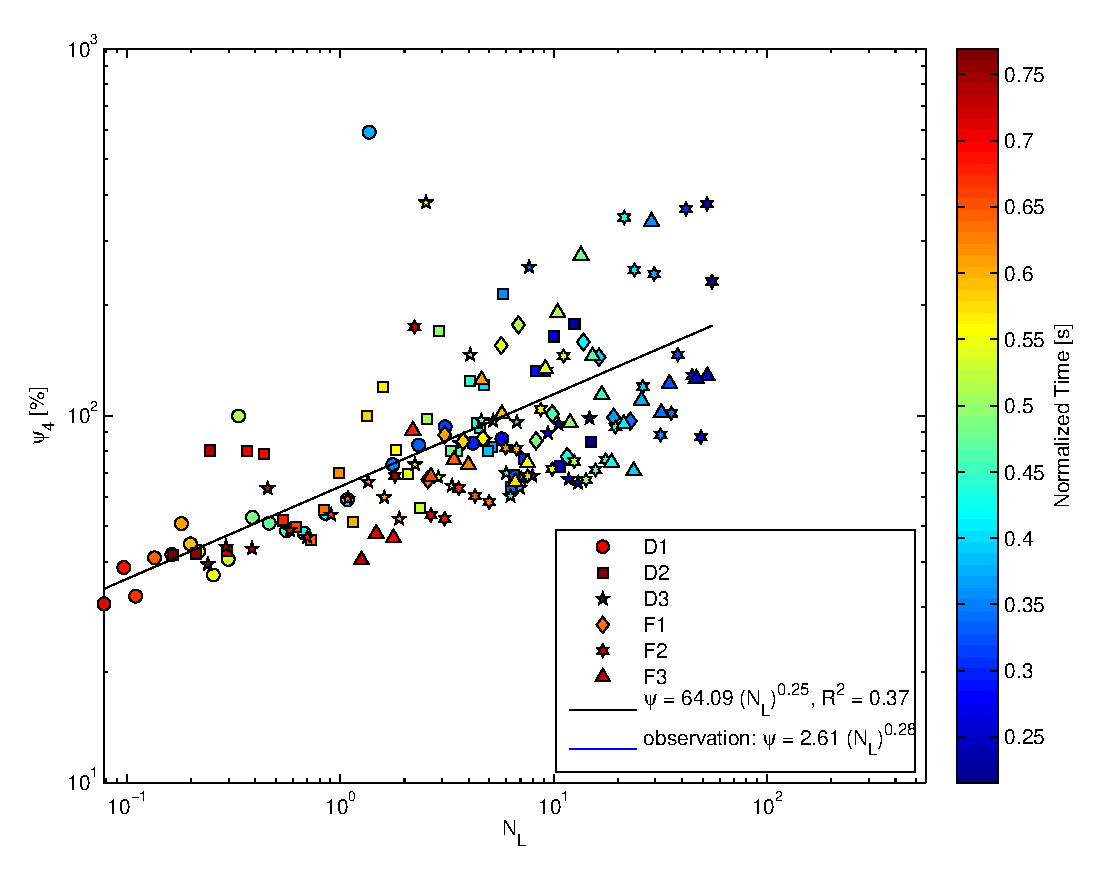
\includegraphics[width=0.49\linewidth]{Figures/phi4nl}
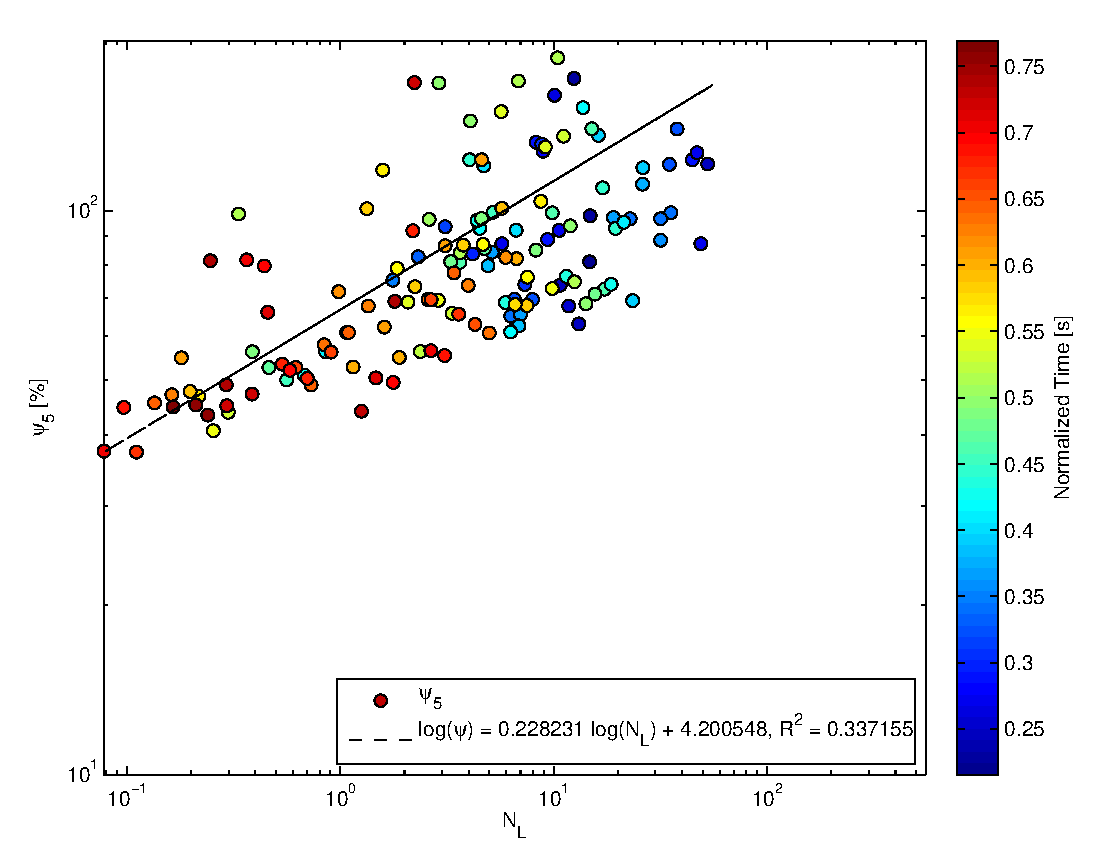
\includegraphics[width=0.49\linewidth]{Figures/phi5nl}
\caption{Scatter plot of the homogeneous mixing degree vs the transition scale number. All the cases are shown in one figure. From left to right, up to bottom are $\psi_1$, $\psi_2$, $\psi_3$ and $\psi_4$.\label{fig:mix_degree_nl}}
\end{figure}

\section{Conclusions}\label{conclusion}
In this paper, a series of numerical simulations are performed to study the cloud entrainment and mixing phenomena. Three different configurations are compared with each other to inspect the influence of the initial cloudy shape on the cloud microphysics in the mixing process. The simulation duplicates the configurations in \cite{And04} and \cite{Kumar11} and agrees with their main results. Case 1 corresponds to \cite{And04}, which is aiming to study the final stage of the mixing process. Case 2 tries to mimic the idealized cloud slab in \cite{Kumar11}, presenting a complete view of entrainment and mixing. Case 3 is created by rotating case 2 with $90$ degree clockwise to show the sedimentation effects on the droplet spectrum.

The work described in this paper almost follows the configurations in \cite{Kumar11}. However, due to the Gibb's phenomena of the pseudo-spectral method, there is an inconsistency between the initial profile of cloud droplets and vapor mixing ratio in \cite{Kumar11}, in which an artificial continuous function was used to connect the area of cloudy air and clear air, while the cloud droplets were treated as a simple slab. This inconsistency is not desirable and can be overcome by taking advantage of the high resolution finite difference WENO scheme, which is designed for problems with piecewise smooth solutions containing discontinuities. Therefore, we are able to perform the simulation with the same sharp initial interface for both cloud droplets and the vapor mixing ratio.

All the simulation have been tested in both decaying turbulence and forced turbulence. The thermodynamics, cloud microphysics and mixing diagram are studied to make a comparison between different cases. The transient growth of turbulence kinetic energy due to buoyancy effects in the decaying cases agrees with the observation in \cite{Kumar14}. The spectrum of droplets size and supersaturation implies that the cloudy shape effectively influence the mixing process in decaying turbulence by affecting the reaction time and the size distribution. However, this effect seems to be much smaller in the forced turbulence.

The mixing diagram is then plotted to compare the $R_v^3$-$N_c$ relationship in different cases, which have the same final state with zero liquid water content. The number concentration in case 1 does not change for a long time due to its already diluted configuration. This implies that the initial reductions of number concentration in case 2 and 3 are due to dilution process. Case 2 is performed to duplicate the results in \cite{Kumar14} for radius $15\mu m$ (note that their results were amended in \cite{Kumar16Corr}). Our results disagree the conclusion in \cite{Kumar14} but support their amendment in \cite{Kumar16Corr}, that is the mixing trajectories are not scattered around the homogeneous mixing curve. The configuration of case 3 is the same as case 2 except the direction of the cloud slab. The results infer that the sedimentation will accelerate the mixing to a certain degree when comparing with case 2. Two groups of mixing trajectories are observed in the results of case 3. We interpret the separation of the curves as an indication that the sedimentation will push the particles moving downwards, so as to accelerate the mixing process.

\cite{Jarecka2013}, utilized the DNS results from \citep{And04, And06, And09} to estimate the mixing scenario with a parameter $\alpha$ and merged the $\lambda-\beta$ subgrid scheme \cite{Jarecka2009} with the double-moment LES model \cite{Morrison2008}. Because of the limitations of numerical technology, our study can only address the late stages of the entrainment-mixing process, where the filamentation by large-scale eddies is already less important, and where mixing-evaporation takes place \cite{Jensen1989}. Although care has to be taken when extrapolating the results of our simulations to natural clouds, the quantitative nature of this study provides a guidance for future research of small-scale and microscale processes in clouds. 

It should be kept in mind that there is a major limitation to the approach used in this work. DNS of turbulent flows is limited to much lower Reynolds numbers than that of cumulus clouds. This implies that we will not be able to quantify effects associated with the presence of coherent structures characteristic of high Reynolds number turbulent flows.

\section{Acknowledgements}
The research was supported by the U.S. Department of Energy's Atmospheric System Research(ASR) and Earth System Modeling (ESM) programs and partially by the US Army Research Office under ARO-DURIP Grant W911NF-15-1-0403.
\bibliographystyle{agufull08}
\bibliography{refs}

\end{article}
\end{document}
